\section{Methodology} \label{sec:methodology}
The primary goal to reach when analyzing dune field images is to compute and extract meaningful features, as discussed in \cite{ewing-kocurek-lake-2006,ewing-peyret-kocurek-bourke-2010}. The two main features extracted in this research are the following:

 \begin{description}
 	\item [Orientation] The orientation (both local and global) of a dune field can provide researchers valuable information about climate and wind patterns in the area.
 	\item [Inter dune spacing] The distance between crest-lines also provides valuable information about structure of the dune field.
 \end{description}
 
 There are many potential methods to extract such features, but in this research, a crucial first step is to detect crest-lines in the dune field. Crest-lines are the main prominent features in any dune fields. The are characterized by a distinguishable peaks along a ridge of dunes. Extracting the dune crest-lines is a challenging problem in itself, which is explained in \ref{subsec:challenges}. 

 %In this research, a many different approaches have been attempted, which include an appearance-based approach in \ref{subsection:appearance_based_approach}, an edge-based approach in \ref{subsec:edge_based_detection}, using the Watershed Transform in \ref{subsec:watershed_transform_segmentation_approach}, a gradient orientation based method in \ref{subsec:gradient_orientation_based}, a machine learning approach in \ref{subsec:machine_learning_approach}, and ultimately the mixed gradient and machine learning approach which is explained in \ref{subsec:mixed_ml_gradient_approach}. Finally, the computation of the dune field morphology metrics is explained in section \ref{subsec:dune-field-metrics}.
 
 \subsection{Challenges} \label{subsec:challenges}
 
 Automated detection of crest-lines from satellite images poses many problems. Finding and labeling crest-lines in images in most cases may be a straight forward task for an expert researcher in this field, but quickly becomes a tedious task as the amount of data increases. The need for automated detection of such features is very apparent. However, there are regions where dune fields are complex and dense, making automated dune detection a much more difficult task.
 
 Generally, a crest-line is visible by the fact that it has a sunlit side, and a shaded side. Areas in the image where a bright region meets with a darker region are typically good candidates for potential crest-lines. This important criteria assumes that the sun's orientation is roughly perpendicular to the dune ridges. When ridges approach a parallel orientation to the sun's orientation, the crest-lines become less pronounced. The problem is evident as shown in Figure \ref{fig:difference_between_dune_field_types}, from linear dunes in the Kalarahi (\ref{fig:difference_between_dune_field_types_kalahari}) to the complex structure of the White Sands dune field (\ref{fig:difference_between_dune_field_types_whitesands}).
 
 \begin{figure}
 	\centering
 	\begin{subfigure}{0.48\textwidth}
 		\centering
 		%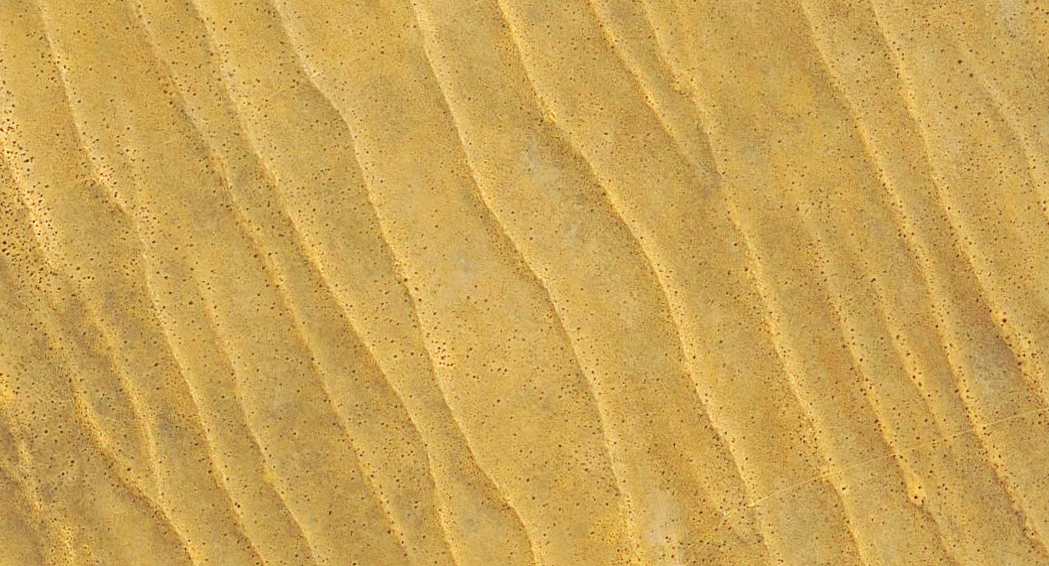
\includegraphics[width=\linewidth]{figures/kalahari}
 		\caption{Kalahari: Linear dune system}
 		\label{fig:difference_between_dune_field_types_kalahari}
 	\end{subfigure}
 	\begin{subfigure}{0.48\textwidth}
 		\centering
 		%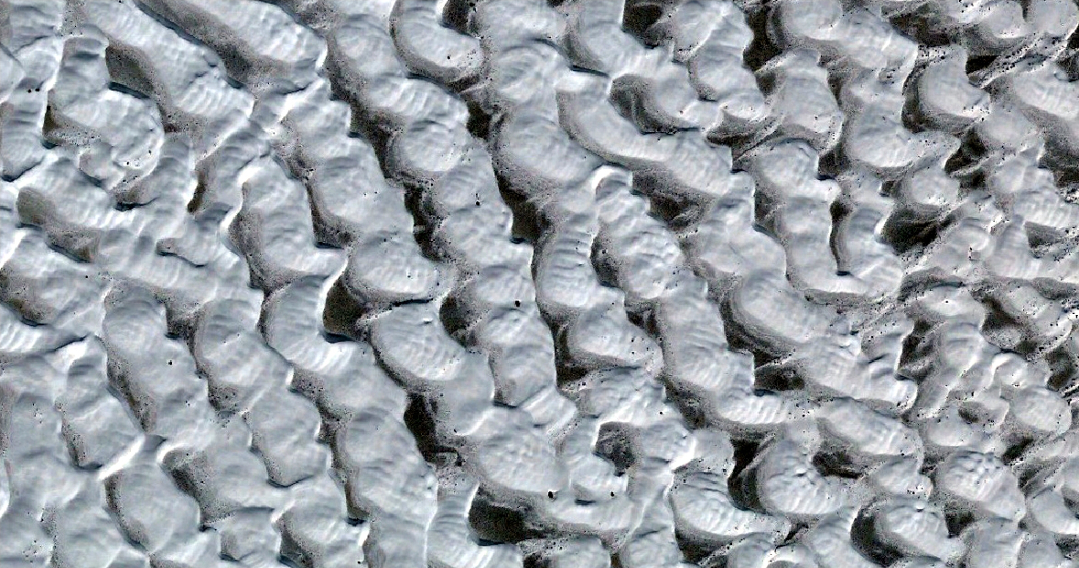
\includegraphics[width=\linewidth]{figures/whitesands}
 		\caption{White Sands: Complex dune system}
 		\label{fig:difference_between_dune_field_types_whitesands}
 	\end{subfigure}
 	
 	\caption{The variation in dune patterns such as \subref{fig:difference_between_dune_field_types_kalahari} linear, or \subref{fig:difference_between_dune_field_types_whitesands} complex, and the sun orientation and illumination effects on the resulting satellite images.}
 	\label{fig:difference_between_dune_field_types}
 \end{figure}
 
 Another important feature present dune crest-lines are the edges between the sunlit side and the shaded side. One assumption is that crest-lines produce relatively stronger edges than other areas of the image. This assumption was the principle guiding criteria in \cite{2015_automated_mapping_of_linear_dunefield}. However, the strength of the edge depends on many factors:
 
  \begin{enumerate}
	\item The sharpness of the actual dune ridge: dune which have sharper crest-lines will undoubtedly produce stronger, more defined edges on the satellite images.
	\item The sun's orientation and time of day: As the sun approaches the horizon, the sunlit and shaded sides of the dunes become more defined. Inversely, when the sun is higher in the sky, shadows become less pronounced. Also, as discussed previously, the orientation relative to the dune field itself affects the strength of the edges.
	\item Scale, noise and resolution of the image can all affect the strength of edges.
  \end{enumerate}

Understanding the issues with the gradients of the key problem of this research. As shown in Figure \ref{fig:patches}, the pixel values and gradient magnitudes (edge strength) can vary greatly in each region. One inclination is to select strong gradients in an image as candidates for crest-lines (as done in \cite{2015_automated_mapping_of_linear_dunefield}). However, the gradients of crest-lines are not always larger than the gradients of valleys or the shadows. 

In Figure \ref{fig:patches}, a plot of the intensity, gradient magnitudes, and gradient orientations along a cross section of a crest-line is shown. In the sample image patches \ref{fig:kalahari_patch}, \ref{fig:skeletoncoast_patch}, \ref{fig:wdc_patch}, the intensity values of the pixels along the direction shown are plotted in blue in Figures \ref{fig:kalahari_patch_plot}, \ref{fig:skeletoncoast_patch_plot}, \ref{fig:wdc_patch_plot}, the gradients magnitudes are shown in red, and the gradient orientations are shown in a dotted black line. 

\begin{figure}
	\centering
	\begin{subfigure}{0.15\textwidth}
		\centering
		%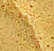
\includegraphics[width=\linewidth]{figures/kalahari_patch}
		\caption{}
		\label{fig:kalahari_patch}
	\end{subfigure}
	\begin{subfigure}{0.15\textwidth}
		\centering
		%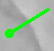
\includegraphics[width=\linewidth]{figures/kalahari_patch_arrow}
		\caption{}
		\label{fig:kalahari_patch_arrow}
	\end{subfigure}
	\begin{subfigure}{0.65\textwidth}
		\centering
		%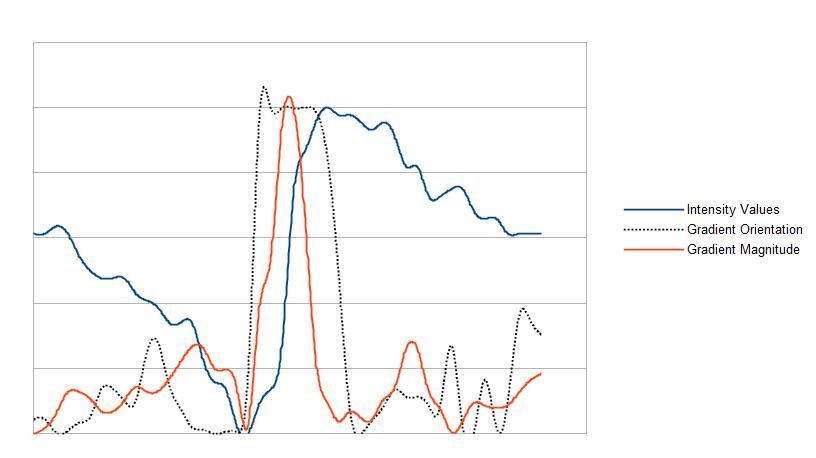
\includegraphics[width=\linewidth]{figures/kalahari_patch_plot}
		\caption{}
		\label{fig:kalahari_patch_plot}
	\end{subfigure}
	
	\begin{subfigure}{0.15\textwidth}
		\centering
		%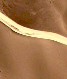
\includegraphics[width=\linewidth]{figures/skeletoncoast_patch}
		\caption{}
		\label{fig:skeletoncoast_patch}
	\end{subfigure}
	\begin{subfigure}{0.15\textwidth}
		\centering
		%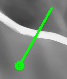
\includegraphics[width=\linewidth]{figures/skeletoncoast_patch_arrow}
		\caption{}
		\label{fig:skeletoncoast_patch_arrow}
	\end{subfigure}
	\begin{subfigure}{0.65\textwidth}
		\centering
		%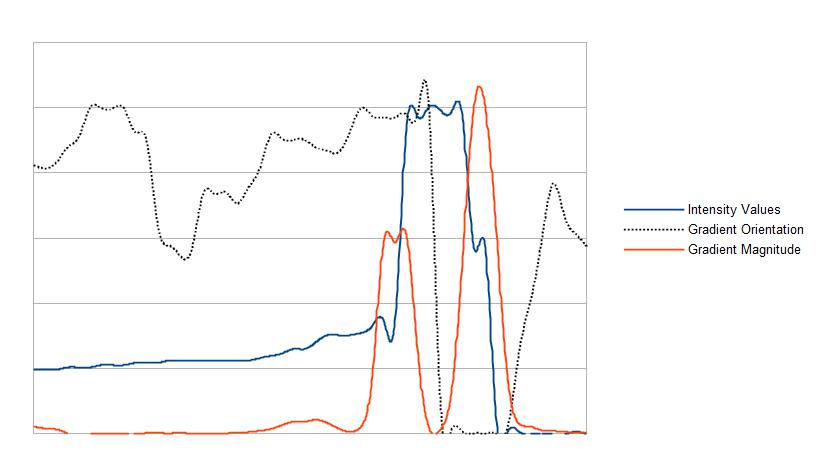
\includegraphics[width=\linewidth]{figures/skeletoncoast_patch_plot}
		\caption{}
		\label{fig:skeletoncoast_patch_plot}
	\end{subfigure}
	
	\begin{subfigure}{0.15\textwidth}
		\centering
		%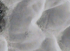
\includegraphics[width=\linewidth]{figures/wdc_patch}
		\caption{}
		\label{fig:wdc_patch}
	\end{subfigure}
	\begin{subfigure}{0.15\textwidth}
		\centering
		%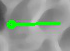
\includegraphics[width=\linewidth]{figures/wdc_patch_arrow}
		\caption{}
		\label{fig:wdc_patch_arrow}
	\end{subfigure}
	\begin{subfigure}{0.65\textwidth}
		\centering
		%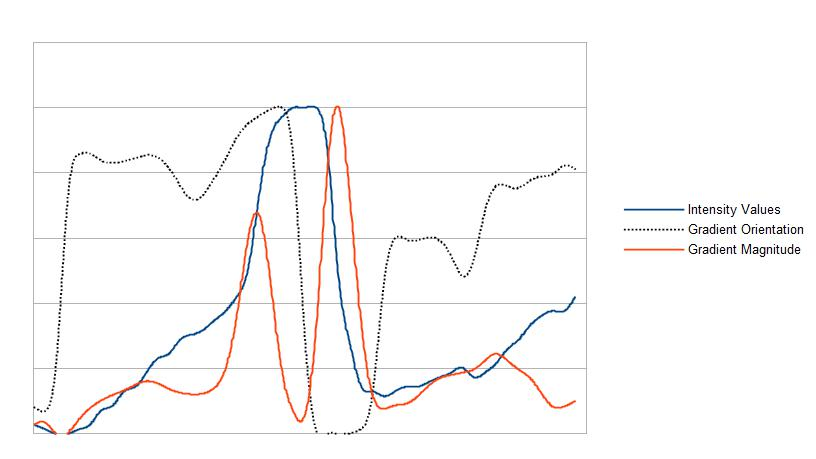
\includegraphics[width=\linewidth]{figures/wdc_patch_plot}
		\caption{}
		\label{fig:wdc_patch_plot}
	\end{subfigure}
	\caption{Illustration of the intensity, gradient magnitudes, and gradient orientations, plotted along a path crossing a dune crest-line: \subref{fig:kalahari_patch}, \subref{fig:skeletoncoast_patch},\subref{fig:wdc_patch} a sample image patch from Kalahari, Skeleton Coast, and White Sands regions, \subref{fig:kalahari_patch_arrow}, \subref{fig:skeletoncoast_patch_arrow}, \subref{fig:wdc_patch_arrow} the direction of the pixel samples plotted in \subref{fig:kalahari_patch_plot}, \subref{fig:skeletoncoast_patch_plot}, \subref{fig:wdc_patch_plot} containing the intensity, gradient magnitude and orientations values along the sampled direction. }
	\label{fig:patches}
\end{figure}

Typically, a peak in intensity values of the pixels is present, representing the sunlit side of a dune. Inevitably, this will produce two peaks in the gradient magnitude on both sides of the intensity peak. One of them represents the true crest-line of a dune, while the other can either be the shadow cast by the dune, or the bottom valley of the dune. The main difference between the two peaks, other than their gradient magnitude, is the fact they are almost always in opposite orientations. One peak is going from dark to bright, the other from bright to dark. If the sun's orientation relative to the dune field is known, then choosing the correct peak is trivial. When the orientation is unknown, choosing the correct peak becomes a challenging problem. 

In \cite{2015_automated_mapping_of_linear_dunefield}, the assumption was made that the weaker of the two edges can be filtered out, claiming that the larger peak is the crest-line, which is valid in the Kalahari image patch in Figure \ref{fig:kalahari_patch_plot}. However, the gradients produced by crest-lines may or may not be larger than their cast shadows, or the valleys. A clear example is shown in Figure \ref{fig:skeletoncoast_patch_plot}. In this scenario, the true crest-line is actually represented by the first gradient peak. The second peak is in fact produced by the shadow of a different dune.

Another interesting challenge is found in the images themselves. The correct crest-line cannot easily be determined by simple observation. A person presented with the image patch shown in \ref{fig:skeletoncoast_patch} would most likely not be able to determine with certainty which one of the edges represents the true crest-line. The obvious solution is to know the orientation of the sun relative to the dune field, but that may not always be possible.

All the challenges listed above need to be addressed in order to accurately and reliably detection dune crest-lines. In the next section, the overall process flow of the crest-line detection application is presented.

\subsection{Overall Process Flow}

In this research, many different approaches were attempted and compared to extract meaningful features from the images and compute the appropriate morphological properties of the dune fields. The overall process flow of detecting crest-lines can be represented as a five stage process:

 \begin{figure}[H]
 	\centering
 	%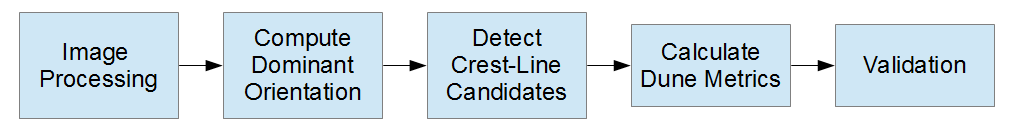
\includegraphics[width=\linewidth]{figures/flow1}
 	\caption{The overall process flow for general dune detection. The five steps include image processing, dominant orientation computation, crest-line candidate detection, calculations of dune metrics, validation of crest-line candidates.}
 	\label{fig:main_flow}
 \end{figure}

\subsubsection*{Image Processing}

The pre-processing stage is an important step to normalize and de-noise the input data. Image processing is typically a low level process which attempts to improve image quality, normalize illumination, or remove unnecessary noise from the image. This type of processing will in turn improve higher level feature extraction.

The first step is to insure that the images have roughly the same scale. To enforce scale normalization, the datasets scales were manually selected for appropriate crest-line detection application, and the image resolutions were resized to roughly 1000 pixel in width. The appropriate resolution is chosen based on a few factors:

\begin{itemize}
	\item Source resolution: The selected resolution is limited by the original image's resolution. No extra information can be gained from increasing the source image's resolution.
	\item Processing time: Higher resolution images require much more processing time overall which could be a limitation in a certain application.
	\item Scale selection: If the application's domain is found in a higher scale space, a higher resolution may not necessarily be required.
\end{itemize}

In this application, the goal is to detect the major crest-line, which is a higher scale domain, which means a higher resolution image is not a necessity. However, the parameter selection in these processes are dependent on the resolution and scale of the images. In future work, the dominant scale of the crest-lines could be determined automatically to improve the robustness of the algorithms.

The next step in the process is to convert the images to gray scale. The images in the terrestrial, and Ganges datasets (described in section \ref{subsec:terrestrial_dataset} and \ref{subsec:mars_dataset}) are color images by default. Although color processing of these images has not extensively been tested as part of this study, it is arguable whether using color information would improve the detection results. By converting the images to gray scale, an added benefit of normalizing the images across many region is implicitly enforced. Finally, the conversion process turns the three channel image into a single channel image which improves overall processing performance.

The final preprocessing step is to improve the image quality with low-pass filters. Many of the algorithms in this method rely on gradient information. Therefore, to extract the meaningful gradients, removing the highest frequencies (which in typically are responsible for noise), while preserving the lower scale or more desirable gradients. Two main popular filters are utilized. The median filter, introduced in \cite{huang_median_filtering_algorithm}, is applied first to remove grain and salt and pepper noise while preserving important edges. In some cases, median filtering also helps remove some smaller scale objects such as bushes, trees, rocks, and other features which are indistinguishable from satellite images. Following this, the standard Gaussian filter is applied which removes the remaining high frequency noisy signals from the image.

An important aspect to note is the size of the filter masks, which is heavily dependent on the resolution of the input image. We found that in most cases, for images around 1000 pixels in width, a \emph{sigma} value of approximately 1.5 and mask size of 7 by 7 was sufficient for this application. Once the image has been preprocessed, the gradients can be computed and saved for future use. Gradients can be computed by taking the first derivative of the image, using the popular Sobel operator.

An optional additional step is to apply histogram equalization to the image \cite{digital_image_processing_book}. Poorly illuminated or low contrast images greatly benefit from histogram equalization, because it stretches the contrast of the image in a consistent way. This in turns also helps in the extraction of edges, and improves determination of the dominant gradient orientation.

For the most part, the image processing step is common to most approaches proposed in this section. Some approaches require more or less pre-processing, but typically the processing is applied to each image before any detection is attempted.

\subsubsection*{Computing the Dominant Orientation} 
The dominant orientation is defined as the orientation of the gradients of crest-lines for the entire dune field. Computing the dominant orientation is an essential process in order to determine which gradients correspond to the actual crest-lines. This determination greatly improves the ability to filter out false positive candidates. In datasets where the sun's azimuth is known, the dominant orientation can be directly calculated using the sun's orientation. However, in cases where this information is not provided, the dominant orientation must be computed automatically. Sections \ref{subsec:dominant_orientation_k_means} and \ref{subsec:dominant_orientation_histogram_of_gradients} offer two main approaches to computing the dominant orientation.

\subsubsection*{Detecting Crest-Line Candidates}
The general crest-line candidate detection step extracts candidate segments which are most likely candidates for crest-lines. There are many potential methods to extract segments from the satellite images. The approaches explained in this section include appearance-based methods, which use the pixel values to extract crest-lines (\ref{subsection:appearance_based_approach} and \ref{subsec:watershed_transform_segmentation_approach}), gradient-based methods, which compute the derivatives of the images to extract the gradients (\ref{subsec:edge_based_detection} and \ref{subsec:gradient_orientation_based}), frequency domain methods (\ref{subsec:frequency_domain_approach}), and finally machine learning methods (\ref{subsec:machine_learning_approach} and \ref{subsec:mixed_ml_gradient_approach}). 

Each of these methods have slightly different processing flows but ultimately provide a way to extract candidate crest-lines. Once candidates have been extracted, some post-processing is often applied to reject some segments which do not fit the criteria of dune crest-lines. Rejected segments are typically filtered by length (too short), shape (too much curvature), weakness of gradients, or other factors. The remaining segments can also be smoothed in order to provide less noisy segments.

\subsubsection*{Dune Metrics Calculations}
Computing the dune metrics is the process of extracting the various geomorphological properties of the dune fields from the detected crest-lines. The two main metrics computed in this research are the orientation and inter-dune spacing. The reason these are the main important features is because they actually provide a large amount of information for researchers on the behavior of the dune fields. Additionally, they are fairly trivial to compute once dune crest-line segments have been extracted. Within the framework of this research, they can serve also as a proof of concept and validation of each crest-line detection method. 

In future work, other metrics, features, and properties could be computed, depending the specific research needs. The process of computing these metrics is discussed in detail in section \ref{subsec:dune-field-metrics}.

\subsubsection*{Validation}
The validation process evaluates the quality of each crest-line detector. In order to perform the validation, a dataset of ground truth is provided with each image. The main result metrics of the validation process are the precision and recall. Precision is the percentage of correctly identified crest-lines within the set of candidates. Recall is defined to be the percentage of correctly detected crest-lines from the ground truth. 

In addition, the validation process compares the results of the dune metrics calculations from the detected crest-lines and the ground truth. The same process of computing the dune metrics is also computed on the ground truth, and compared side-by-side with the detected crest-lines. The process is described in detail in section \ref{subsec:evaluation}.

The next section presents the first approach which is an appearance-based method.



 \subsubsection*{Dominant Orientation Determination} \label{subsec:dominant_orientation}
 
 Computing the dominant orientation of the dune field is an important step in the process. The dominant orientation is the overall gradient direction of the crest-lines to be detected. This process can help determine the average orientation of the dune field as well. 
 
 An important point to make is that this process could be optional if the dominant orientation is known \emph{a priori}. Working with a dataset where the values are known improves the overall results of detection and enables skipping of this step. In cases where this information is unknown, or unavailable, automated dominant orientation determination is a potential solution.
 
 Typically, there exists a gradient peak at the crest-line peak of the dunes (although this may not always be the case for less pronounced dunes). The direction of the gradient should agree with the overall dominant orientation of the dune field. Computing the dominant orientation of the field can be challenging in many cases because dunes typically have two major orientations, which are opposite directions. This phenomenon is clearly illustrated in Figure \ref{fig:computing_dominant_orientation}. The true crest-line peak, where the sunny side meets the shaded side is one gradient (Figure \ref{fig:true_dominant_orientation_image}). At the foot of the dune, where the shaded returns to light, a second gradient will be present, whom has an opposite direction (Figure \ref{fig:false_dominant_orientation_image}).
 
 Histograms of gradient directions can be used to determine the true orientation. Histograms have been used for many processes and applications including \cite{lowe_sift_paper, dalal_histogram_oriented_gradients_human_detection, hu_gradient_field_descriptor}. Quantizing the space allows us to split edges according to their orientation, where each bin in the histogram represents an edge orientation. Each bin then covers an angle of $\frac{2\pi}{N}$radians, where \emph{N} is the number of bins. Each bin of the histogram is weighed by the magnitude of edges. Once the histogram is constructed, peaks in the magnitude will help determine the dominant orientation ($\varPhi$) of the dune crest-lines. The approach poses three main problems:
  
  \begin{enumerate}
  	\item Determining \emph{N}: In practice, a larger value for \emph{N} has shown to provide finer grain resolution which improves dominant orientation determination. In Figure \ref{fig:computing_dominant_orientation}, a value of $N=18$ is used (resulting in bins of $20\degree$ width).
  	\item Multiple Peaks: Often, images may have multiple peaks in the histogram, but only one of the peaks should represent the true dominant orientation of the crest-lines. As noted in \cite{2015_automated_mapping_of_linear_dunefield}, the histograms typically have a strong bimodal distribution, which is very apparent in Figure \ref{fig:dominant_orientation_histogram}.
  	\item Global Solution: The computed dominant orientation is global to the image, which may not be optimal in cases of complex dune structures. A better solution would be to compute the dominant orientation in a local area of the image, to account for local shifts in orientation.
  \end{enumerate}
  
  One assumption made is that the bin with the largest value represents the orientation of the crest-line edges. Although this assumption holds for many cases, it is not always the case. The Skeleton Coast test image provides a good example of this case in Figure \ref{fig:computing_dominant_orientation}. In this particular case, the are two major peaks in the histogram, where the stronger is not the part of the crest-line edge group, and the weaker one is. Choosing the higher peak will cause invalid crest-lines to be chosen. In order to determine which peak best represents the crest-line edge group, some normalization can be applied. The normalization process begins by computing the mean vector of the gradients from the edge image as follows:
  
  \begin{equation}
  \hat{\mu}\left\langle \bar{x},\bar{y}\right\rangle =\left\langle \frac{\sum_{i=0}^{P}\delta_{x_{i}}}{P},\frac{\sum_{i=0}^{P}\delta_{y_{i}}}{P}\right\rangle 
  \end{equation}
  
  where \emph{P} is the total number of detected edges from the Canny edge detector, $\delta_{x_{i}}$ and $\delta_{y_{i}}$ are the \emph{x} and \emph{y} gradient component of the \emph{i}\textsuperscript{th} point. The mean orientation is computed from the mean vector as:
  
  \begin{equation}
\bar{\theta_{\mu}}=\arctan\left(\frac{\mu_{\bar{y}}}{\mu_{\bar{x}}}\right)
  \end{equation}
  
  The gradients are then normalized by simply subtracting the mean vector from each gradient:
  
  \begin{equation}
\dot{\delta}\left(x_{i},y_{i}\right)=\left(\delta_{x_{i}}-\mu_{\bar{x}},\delta_{y_{i}}-\mu_{\bar{y}}\right)
  \end{equation}
  
  The normalized orientation $\dot{\theta_{i}}$ can be computed:
  
  \begin{equation}
  \dot{\theta_{i}}=\arctan\left(\frac{\dot{\delta_{y_{i}}}}{\dot{\delta_{x_{i}}}}\right)
  \end{equation}

  \begin{figure}
  	\centering
  	\begin{subfigure}{0.48\textwidth}
  		\centering
  		%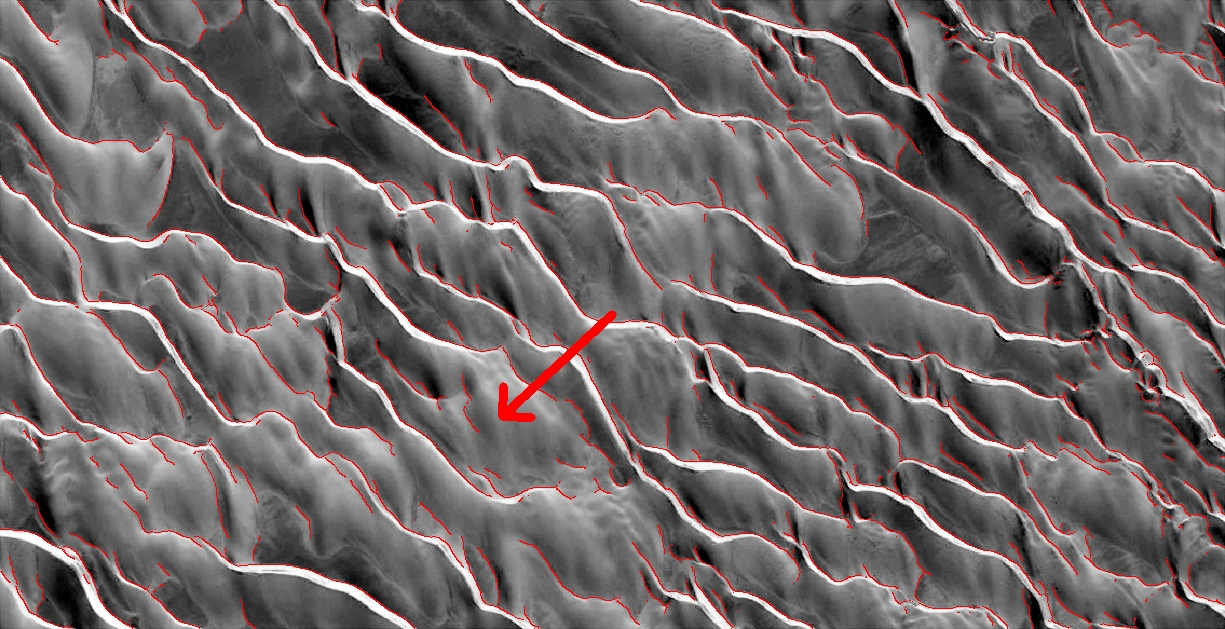
\includegraphics[width=\linewidth]{figures/dominant_orientation_false}
  		\caption{Non-Crest-line Edges}
  		\label{fig:false_dominant_orientation_image}
  	\end{subfigure}
  	\begin{subfigure}{0.48\textwidth}
  		\centering
  		%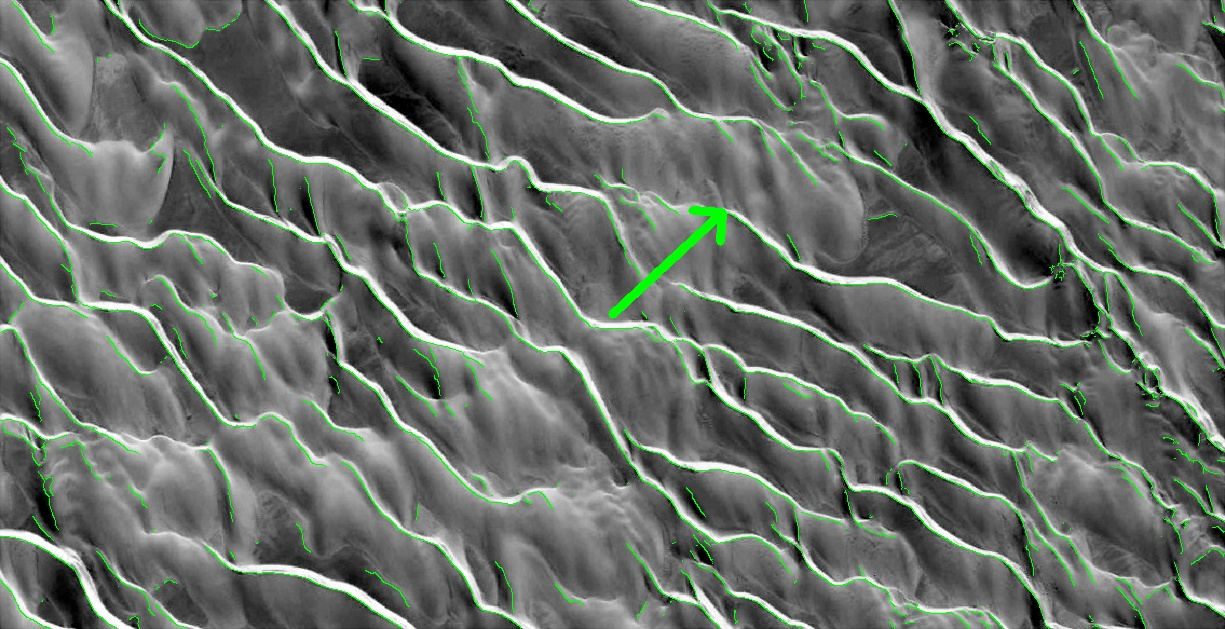
\includegraphics[width=\linewidth]{figures/dominant_orientation_true}
  		\caption{Crest-line Edges}
  		\label{fig:true_dominant_orientation_image}
  	\end{subfigure}
  	\begin{subfigure}{\textwidth}
  		\centering
  		%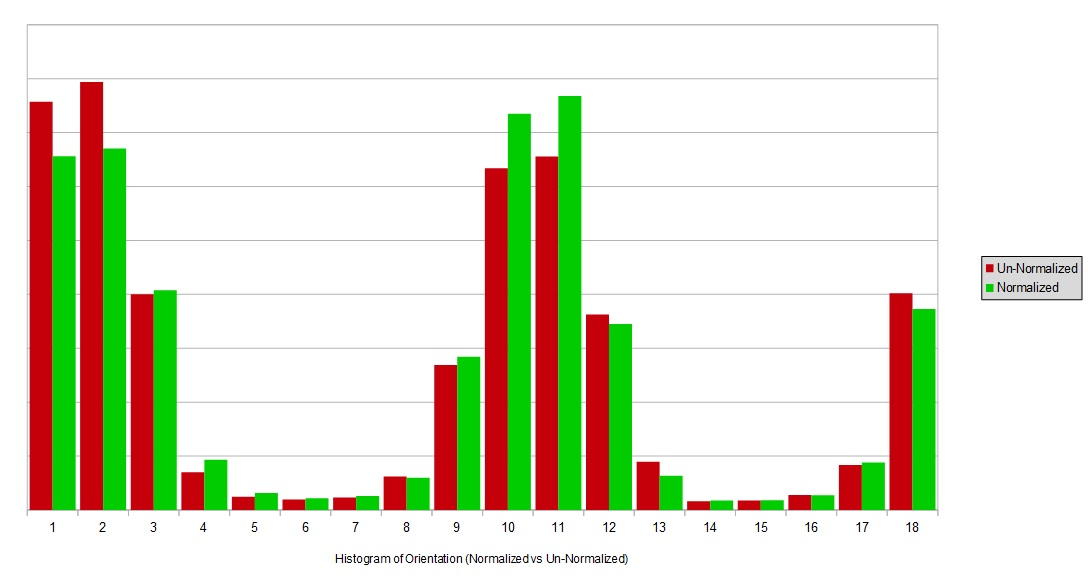
\includegraphics[width=0.8\linewidth]{figures/dominant_orientation_histogram}
  		\caption{Histogram of Gradient Orientations}
  		\label{fig:dominant_orientation_histogram}
  	\end{subfigure}
  	\caption{Results of unnormalized (red) and normalized (green) histograms of gradients orientations ($N=18$), where each represents a $20\degree$ slice. The histogram contains two major peaks, but the crest-line is the weaker of the two peaks. \subref{fig:false_dominant_orientation_image} Edges which belong to the dominant orientation which are invalid crest-lines. \subref{fig:true_dominant_orientation_image} With normalization, the true crest-lines now have the higher overall magnitude. \subref{fig:dominant_orientation_histogram} The 18 bin histogram of gradients with and without normalization.}
  	\label{fig:computing_dominant_orientation}
  \end{figure}
  
  To determine which bin the \emph{i}\textsuperscript{th} edge point belongs to, we simply calculate $\left\lceil \frac{\dot{\theta_{i}}\centerdot N}{2\pi}-0.5\right\rceil $,	and increment that bin by the magnitude of the normalized gradient	by $\sqrt{\dot{\delta}_{x_{i}}^{2}+\dot{\delta}_{y_{i}}^{2}}$. In essence, this normalization process removes the uneven skew of the gradients in the overall image. Removing this skew allows true crest-line edges to be fairly compared with other stronger edges. As shown in Figure \ref{fig:computing_dominant_orientation}, the normalization process softens the stronger dominant edge and enhances the true crest-line edges. This process enables true crest-lines to be accurately determined in images where the valleys of dunes are sharp and contain strong edges.
  
  Once the histogram is computed and normalized, the dominant orientation vector $\hat{\theta_{dom}}$ is determined by averaging the gradients belonging to the histogram bin with the highest value. With the dominant orientation knowledge acquired, candidate crest-line dunes can be detected.
  


\subsection{Gradient Orientation-Based Approach} \label{subsec:gradient_orientation_based}
In this approach, we used knowledge learned from a previous gradient based approach, but focus on the orientation component of the gradients rather than the magnitude. The overall flow of the approach is shown in Figure \ref{fig:flow_gradient_orientation}. 

\begin{figure}[H]
	\centering
	%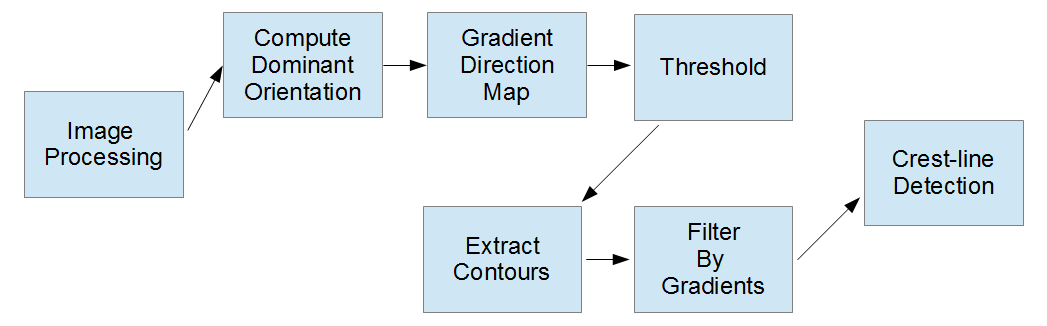
\includegraphics[width=\linewidth]{figures/flow_gradient_orientation}
	\caption{The process flow of the gradient orientation-based approach. The image is first preprocessed for optimal gradient computation, and the dominant orientation is computed. The gradient direction map is then computed and thresholded to preserve all gradients which \emph{agree} with the dominant orientation. The resulting binary image is a good candidate for contour extraction, which are subsequently filtered based on gradient orientation and magnitude. The resulting output is the detected crest-lines segments. }
	\label{fig:flow_gradient_orientation}
\end{figure}

In section \ref{subsec:edge_based_detection}, we learned that the dominant orientation of the dune field could be determined based on the derivatives of the image. In that approach, we used the gradient magnitudes to find major crest-line edges, and filtered out edges which do not \emph{agree} with the dominant orientation of the gradients. Using edges provides good localization but is prone to discontinuity of edge segments.

In contrast, this approach uses the gradient orientations of each pixel to find crest-lines. As stated previously, dunes have a bright and shaded side. Gradients in the bright and shaded sides of the dune have a tendency to point towards the crest-line.

The dominant orientation explained in section \ref{subsec:edge_based_detection} is an important feature to consider in this approach. An aspect of the dominant orientation that was not discussed previously is the fact that by definition, the dominant orientation will always point from the shaded area of the dune towards the sunlit area. This phenomenon is due to the gradient operator. Subtracting a dark pixel (lower value) from a bright pixel (larger value), results in a positive value, which in terms means that the gradients of darker pixels always point towards brighter pixels.

Given this fact, a case can be made for comparing the gradients of each pixel to the dominant orientation vector. All gradient vectors which \emph{agree} with the dominant orientation are then considered to be the shaded sides of a dune, and all gradients which \emph{disagree} with the dominant orientation are therefore part of the sunlit side of a dune. Finally the transition between areas that \emph{agree} and those that \emph{disagree} must be a good potential crest-line candidate.

The concept of \emph{agreement} can be defined mathematically using a simple dot product. Given an dominant orientation defined as a unit length vector $\hat{\delta_{\mu}}$, and the local unit length gradient vector at (i, j) defined as

\begin{equation}
\hat{\delta_{ij}} = \left\langle \frac{\delta_{x_{ij}}}{\sqrt{\delta_{x_{ij}}^2 + \delta_{y_{ij}}^2}}, \frac{\delta_{y_{ij}}}{\sqrt{\delta_{x_{ij}}^2 + \delta_{y_{ij}}^2}}\right\rangle 
\end{equation}

The \emph{agreement} measurement $D_{ij}$ then is simply the dot product:

\begin{equation}
D_{ij} = \hat{\delta_{ij}} \bullet \hat{\delta_{\mu}}
\end{equation}

Since $\hat{\delta_{ij}}$ and $\hat{\delta_{\mu}}$ are both unit-length vectors, the range possible values for $D_{ij}$ is $[-1, 1]$, where positive values represent gradients which \emph{agree} with the dominant orientation, 0 is perpendicular to the dominant orientation, and negative values \emph{disagree} with the dominant orientation. The result of the dot product computed at each pixel is shown in Figure \ref{fig:orientation_based_dot_product}, which we call the gradient direction map.

\begin{figure}
	\centering
	\begin{subfigure}{0.48\textwidth}
		\centering
		%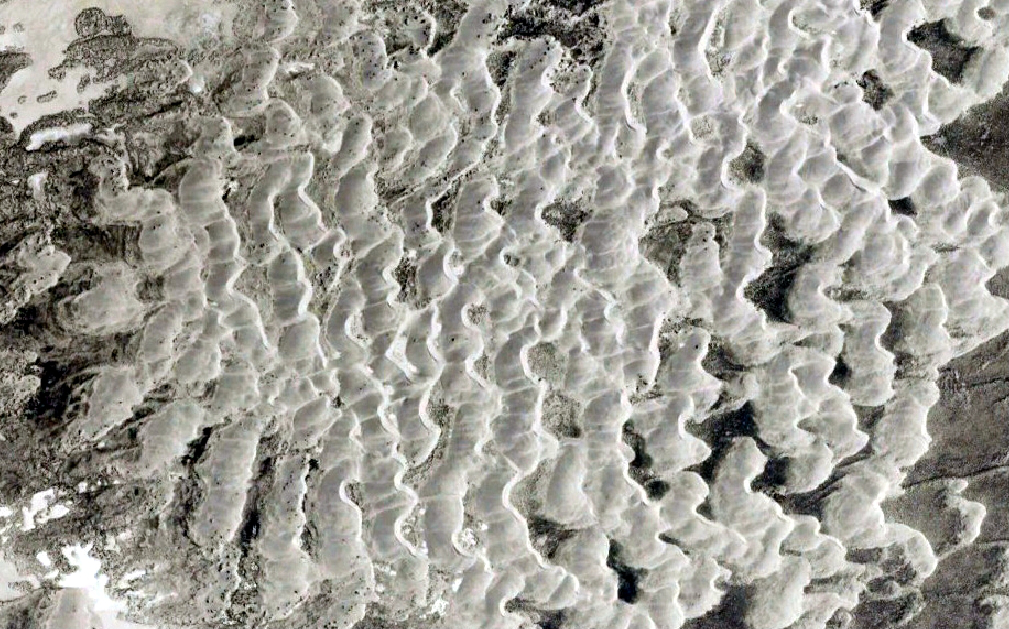
\includegraphics[width=\linewidth]{figures/wdc}
		\caption{WDC}
		\label{fig:orientation_based_wdc}
	\end{subfigure}
	\begin{subfigure}{0.48\textwidth}
		\centering
		%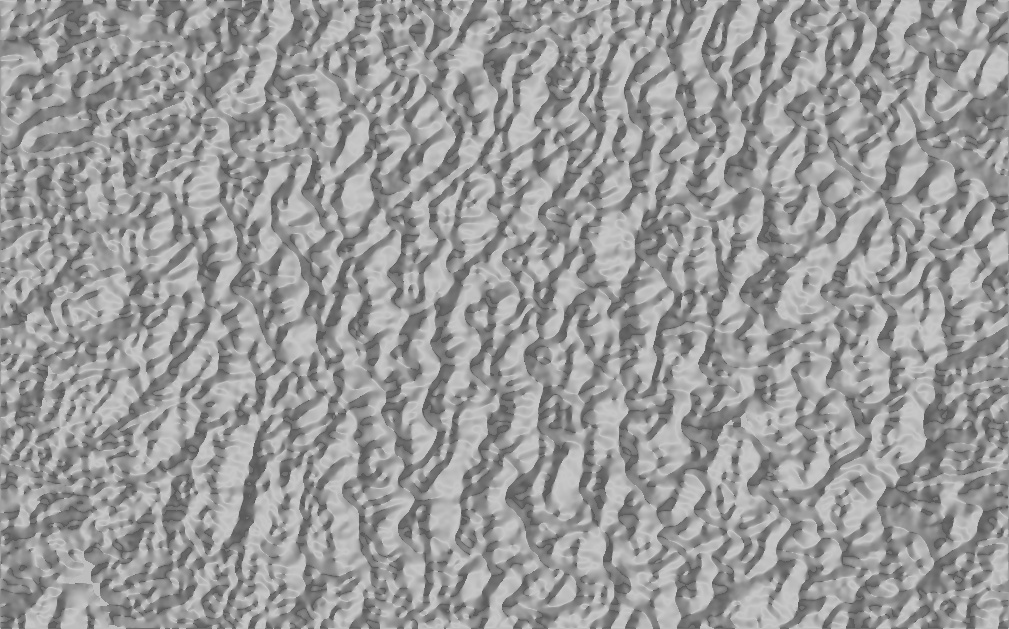
\includegraphics[width=\linewidth]{figures/dot_product}
		\caption{\emph{D}}
		\label{fig:orientation_based_dot_product}
	\end{subfigure}
	\begin{subfigure}{0.48\textwidth}
		\centering
		%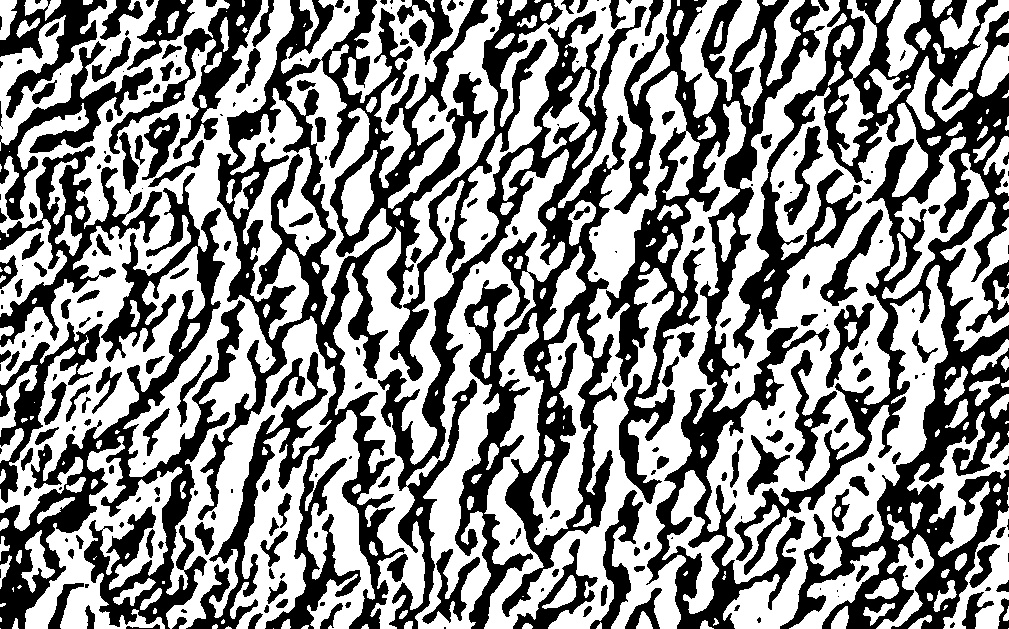
\includegraphics[width=\linewidth]{figures/threshold_dot_product}
		\caption{$\begin{cases}
				1 & D_{ij} > 0\\
				0 & otherwise
			\end{cases}$}
		\label{fig:orientation_based_threshold_dot_product}
	\end{subfigure}
	\begin{subfigure}{0.48\textwidth}
		\centering
		%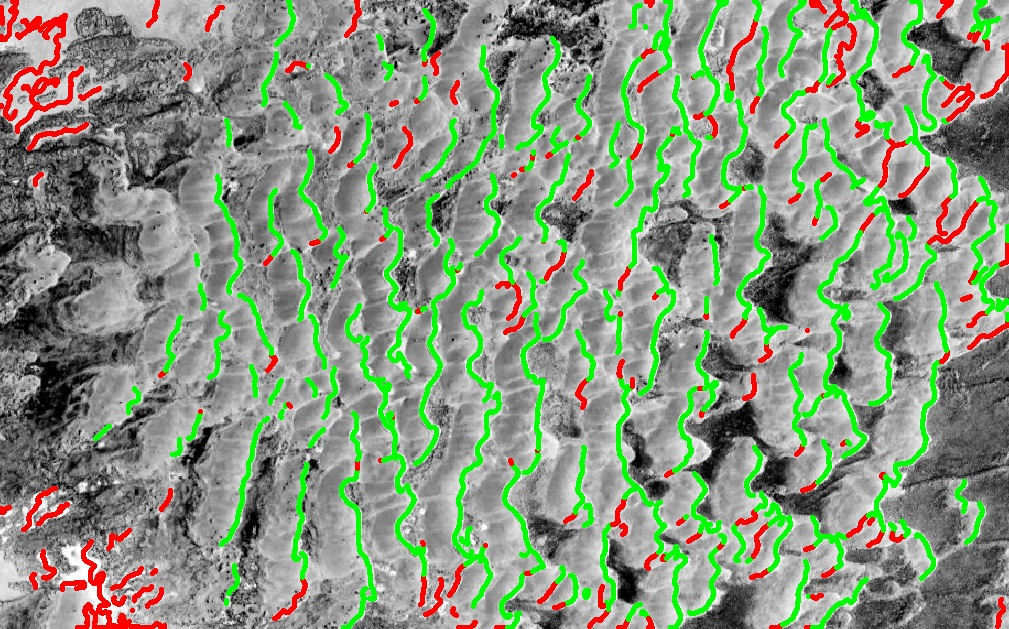
\includegraphics[width=\linewidth]{figures/method_4_results}
		\caption{Result}
		\label{fig:orientation_based_results}
	\end{subfigure}
	\caption{The gradient orientation-based approach illustrated: \subref{fig:orientation_based_wdc} The input image WDC, \subref{fig:orientation_based_dot_product} The gradient direction map \emph{D} computed by taking the dot product of the gradients at each pixel with the dominant orientation, \subref{fig:orientation_based_threshold_dot_product} thresholding the gradient direction map for all dot products greater than 0, \subref{fig:orientation_based_results} the results of crest-line detection using the gradient-orientation based method, where green lines are true positives, and red lines are false positives. }
	\label{fig:orientation_based_process}
\end{figure}

The regions produced by the gradient direction map have been shown to be typically smooth and have good continuity in this application. There appears to be a clear separation between regions in \emph{agreement} and other regions. The separation becomes even clearer when the gradient direction map is thresholded based on the dot product values. In Figure \ref{fig:orientation_based_threshold_dot_product}, a binary image of the gradient direction map is computed by thresholding all dot products above 0.

Once the gradient direction map has been thresholded, the binary image provides well defined regions which allows the use of contours to determine the crest-lines. Contours are extracted in a similar manner as presented in sections \ref{subsection:appearance_based_approach} and \ref{subsec:edge_based_detection}. The contours extracted provide good continuity of the crest-lines, but also contain many elements which are not part of the crest-line. To reject segments of the contour which are not part of the crest-lines, two techniques have been tried.

\subsubsection*{Intensity Based:}

Region contours contain crest-lines segments and non-crest-line segments. In this approach, the algorithm uses intensity values of the pixels along the contours. Segments of the contour which are on brighter regions of the image are considered to be part of the crest-lines. The use of intensity values to determine which segments of a contour are on the actual crest-line may not be an optimal solution, but has provided adequate means of rejecting many false positives.

The main benefit of this approach is that the resulting regions have sharp and defined edges along the dune crest-line, regardless of how sharp an edge is in actuality. In many cases, dunes in the same image may have some sharp edges along the crest-line while others have less defined crest-lines. Using gradient magnitude in areas with poorly defined crest-lines yields poor results, while the gradient direction maps provides a sharper edge and a better estimate of where a crest-line may be. The downside of this method is that not using the gradient magnitude results in poor localization of the actual crest-line.

\subsubsection*{Gradient Magnitude Based:} \label{subsubsec:gradient_magnitude_based_shift}

This algorithm uses the gradient values of the pixels along the contours. The assumption is that segments of the contour with larger gradients are most likely crest-line candidates. 

Using the gradient magnitudes provide much more accuracy in localizing the desired crest-lines. The gradient orientation based approach has an inherent localization problem do the the computation of the gradient orientation and size of the kernel to compute the gradients. The contours will almost always be shifted slightly away from the true crest-line as shown in Figure \ref{fig:orientation_transition_shift}.

Figure \ref{fig:orientation_transition_shift} is the exact same as the plot shown in Figure \ref{fig:kalahari_patch_plot} with the crest-line plotted, and the shift shown. The shift shown is the transition from gradients which \emph{agree} with the dominant orientation ($D_{ij} > 0$) to those which \emph{disagree} with the dominant orientation {$D_{ij} < 0$}. The shift is heavily dependent on the size of the kernel \emph{K} used to compute the gradients.

\begin{figure}
	\centering
	%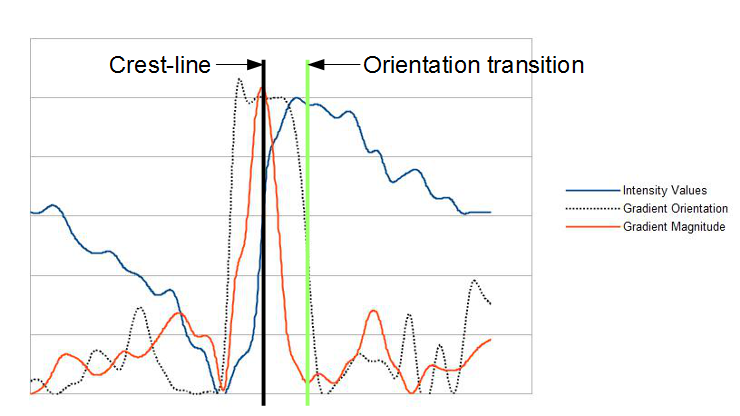
\includegraphics[width=\linewidth]{figures/orientation_transition_shift}
	\caption{The cause of the shift in localization when computing the gradient direction map. The transition from gradients which \emph{agree} ($D_{ij} > 0$) with the dominant orientation almost always happens after the true crest-line due to the size of the kernel \emph{K}.}
	\label{fig:orientation_transition_shift}
\end{figure}

\begin{figure}
	\centering
	\begin{subfigure}{0.48\textwidth}
		\centering
		%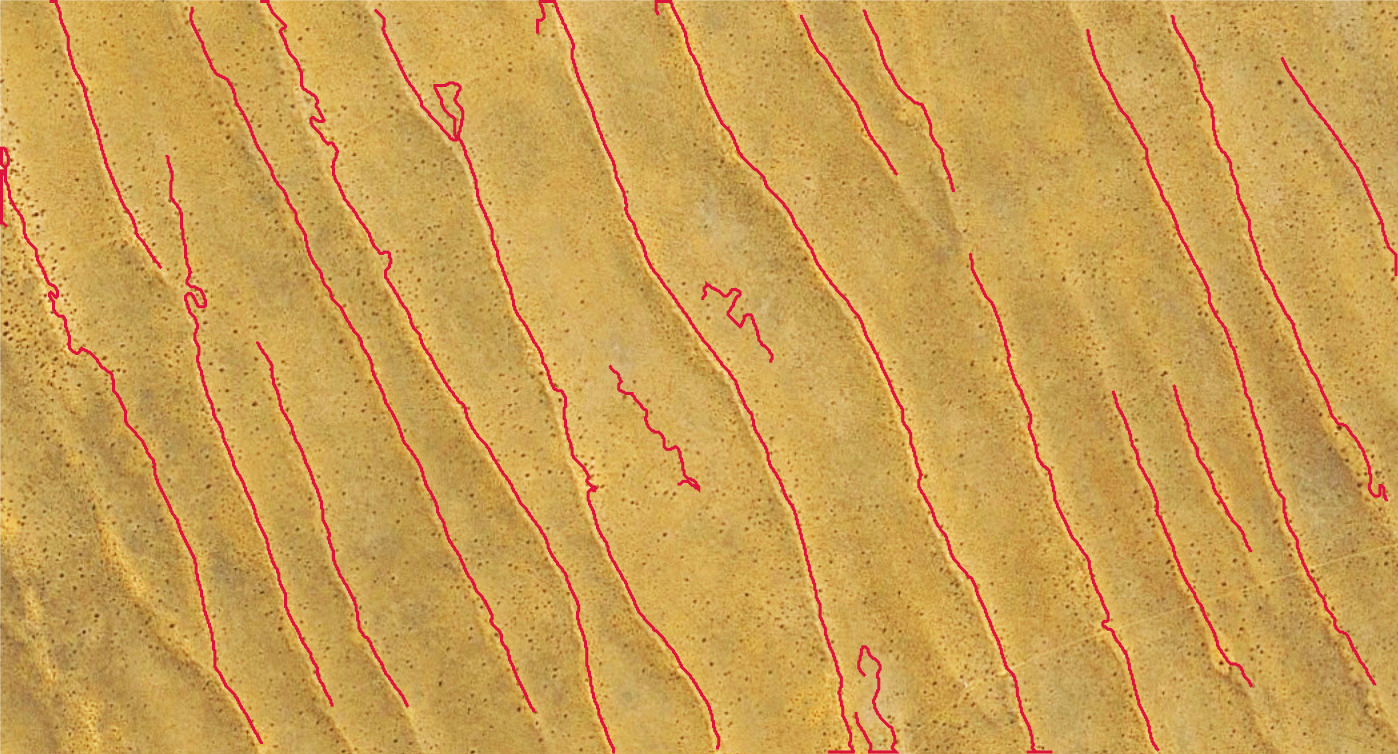
\includegraphics[width=\linewidth]{figures/shift_k_9}
		\caption{$K=9$}
		\label{fig:shift_k_9}
	\end{subfigure}
	\begin{subfigure}{0.48\textwidth}
		\centering
		%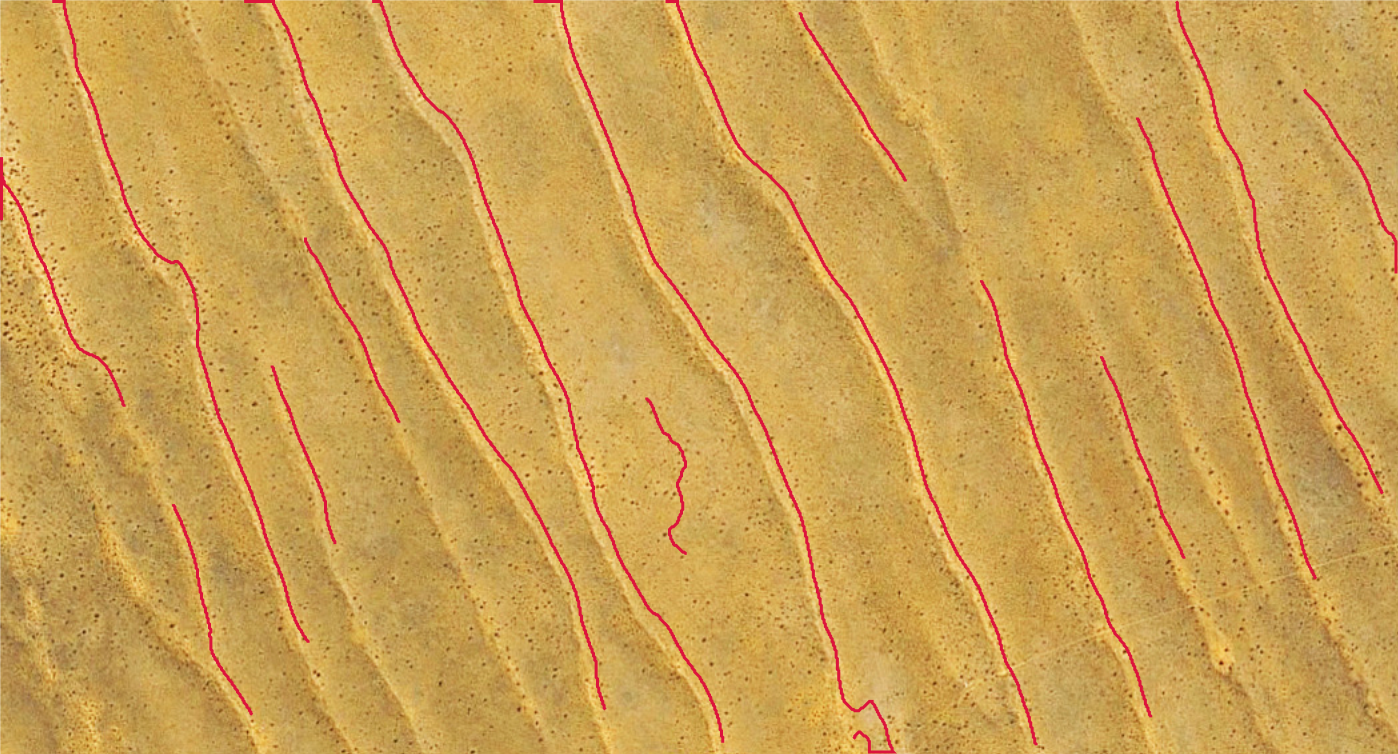
\includegraphics[width=\linewidth]{figures/shift_k_21}
		\caption{$K=21$}
		\label{fig:shift_k_21}
	\end{subfigure}
	\caption{Effects of \emph{K} on the orientation-based approach. In \subref{fig:shift_k_9} a \emph{K} value of 9 is used, which results in better localization at the cost of noisier results, \subref{fig:shift_k_21} a \emph{K} value of 21 produces much smoother results but poor localization. }
	\label{fig:effect_k}
\end{figure}

The contours detected will inevitably land on the orientation transition. As shown in Figure \ref{fig:effect_k}, the parameter \emph{K} will have a tendency to shift the contour lines towards the dominant orientation. In order to improve localization, the contours must be shifted towards to nearest gradient magnitude peak. 

Two methods can be used to shift contours towards the crest-lines. Since the shift is simply dependent on the parameter \emph{K}, a fixed shift can be applied in the opposite direction of the dominant orientation. This approach may be adequate if localization is not critical, but results produced are generally less accurate.

A better solution is to search in the opposite direction of the dominant orientation for the nearest gradient magnitude peak. Each point on the contour can then be shifted by the computed distance to each gradient peak.

\subsubsection*{Parameter Effects}

For this approach, there are relatively few parameters to optimize. The main parameters are:

\begin{enumerate}
	\item The value of \emph{K}, which determines the size of the kernel which computes the gradients. The effects of varying this parameter are shown in Figure \ref{fig:effect_k}. Choosing the appropriate value for \emph{K} depends largely on the scale of the provided image, size and spacing of the dune crests. Larger kernels typically produce smoother results as shown in \ref{fig:shift_k_21}, but result in poor localization.
	\item  The value of \emph{R}, which determines the intensity or gradient magnitude value threshold for rejecting false positives. This is the main value used to determine the the appropriate level of detection. Lower threshold values typically increase the detection rates and false positive rates.
	\item The minimum segment length value, which determines the minimal allowable length for the detected segments. This parameter depends largely on the scale or resolution of the image, and the desired precision of the crest-line detection. Segments which are shorter than the minimum segment length are assumed to be noise, and are filtered out.
	\item The threshold value for the dot product, which determines how closely edges must match the dominant orientation. A value of 0 appears to be adequate in most cases, but it could be adjusted to suit the needs of the application.
\end{enumerate}

Overall, using the orientation information has merit and provides valuable information for crest-line detection. The approach is used and further improved in the approach presented in section \ref{subsec:mixed_ml_gradient_approach}. The next approach presents a traditional machine learning centric approach.



\subsection{Machine Learning Approach} \label{subsec:machine_learning_approach}

In the machine learning approach, the goal is to teach a classifier to recognize crest-lines vs non-crest-lines. A similar approach was implemented in \cite{2006_automated_classification_landform_elements,2007_Machine_Learning_tools_automatic_mapping_mars,2013_sar_image_automated_detection_dune_area,BandeiraMarques,2011_neural_network_based_dunal_landform_mapping,vaz_object_based_dune_analysis}. The goal of this approach is to create a machine learning model using a training dataset, then generate the response map which is the response of the model at each pixel in a given image. Ideally, the responses are high at pixels which contain crest-lines, and low everywhere else. The response map can be thresholded and local maximums can be traced in order to retrieve the crest-lines. The overall flow is illustrated in Figure \ref{fig:flow_ml}.

\begin{figure}[H]
	\centering
	%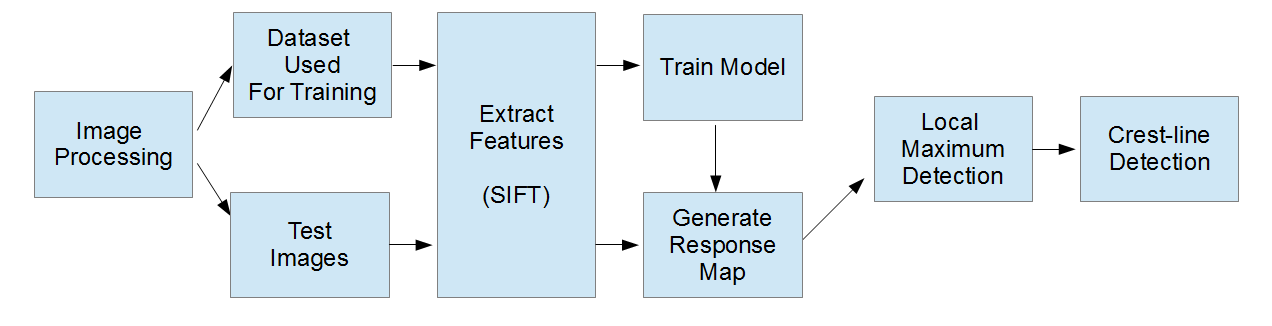
\includegraphics[width=\linewidth]{figures/flow_ml}
	\caption{The process flow of the machine learning approach. The image is first preprocessed, and some training data (samples of crest-lines and non-crest-lines) is reserved to construct the machine learning model. SIFT features are extracted from the training data to train the model to recognize crest-lines. With the model trained, SIFT feature descriptors are computed at each pixel of the remaining test images and are inputted into the trained model to generate the response map. Finally, the local maxima of the response map are detected in order to extract the crest-lines. }
	\label{fig:flow_ml}
\end{figure}

The first step of the process is to appropriately separate the data into training, validation, and test sets in order accurate report the performance of the method. 

\subsubsection{Dataset Creation} \label{subsubsec:dataset_creation}

Machine learning techniques typically require training data to construct the model in order to reliably solve classification problems. This method of training is called supervised learning (\cite{foundations_machine_learning_book,machine_learning_book}). For crest-line detection, we therefore need to split our data into two classes: crest-lines and non-crest-lines. 

For each class, the data also needs to be separated into three sets for training, validation and testing. 

\begin{description}
	\item [Training] The training set is used to construct the model to learn the task at hand.
	\item [Validation] The validation set is used to evaluate the effectiveness of the trained model. Based on the results produced on the validation set, the model parameters can be tuned to produce better results on the validation data.
	\item [Testing] The test set is an independent set used to report the true performance of the model.
\end{description}

In order to build the model for crest-line classification, the first step is to collect the data to build each set. In this application, our datasets included the ground truth for each image set. The ground truth is essentially a binary image with the labeled crest-lines. 

To construct an appropriate dataset for the approach, the set of images is first split into the training/validation and test sets. Half of the images are reserved for testing, and the remaining half is used to training and validation. From the set of training images, the ground truth images are used to extract locations of crest-lines and non-crest-lines. For each image, pixel positions are chosen randomly, if the ground truth at the position contains a crest-line, the pixel location is added to the crest-line set, otherwise it is added to the non-crest-line set. The sampling is optimized so that \emph{N} samples are chosen for each class.

The resulting output is that each training image now has \emph{N} samples of crest-lines, and \emph{N} samples of non-crest-lines. The next step in the process flow is to extract features from each of these samples, which will be used to feed into the model for training and validation.

\subsubsection{Feature Descriptor Extraction} \label{subsubsec:feature_descriptor_extraction}

Once sample locations of crest-lines and non-crest-lines have been selected, descriptors need to be extracted from each sample location. A descriptor is typically a vector of values which describes the local neighborhood around a pixel location (\cite{lowe_sift_paper,1994_good_features_to_track,1998_feature_detection,2007_invariant_features_survey}). The range of possible descriptor types is almost limitless. Descriptors can range from simple pixel values in an image patch, to gradient information, to more sophisticated descriptors such as HOG (Histogram of Oriented Gradients \cite{2007_hog_human_detection}), LBP (Local Binary Pattern \cite{1994_lbp_paper,1996_lbp_paper}), Haar Features (\cite{2001_viola_jones_paper}), SURF (Speeded Up Robust Features \cite{2006_surf}), SIFT (Scale Invariant Feature Transform \cite{lowe_sift_paper}), and many more.

As part of this research, many of those types of features have been investigated. However, the SIFT descriptor has been shown to provide the best overall results. One downside of the SIFT descriptor is the computational requirements of extracting and matching the descriptors. The main reason is the size of a standard SIFT descriptor, which is a vector of 128 floating point values, and becomes computational significant as the number of data samples increase. Despite this downside, SIFT is still an appropriate option since there are no real-time requirements in this application.

\begin{figure}
	\centering
	%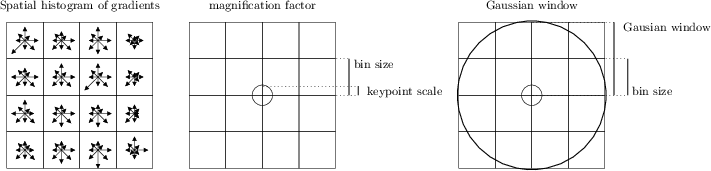
\includegraphics[width=\linewidth]{figures/sift-descriptor}
	\caption{The SIFT descriptor explained. The image patch is split into a 4 by 4 grid, where each cell contains a histogram of gradients of eight directions. The result is a single vector of 128 floating point values. Source of the image: \underline{http://www.vlfeat.org/api/sift.html}}
	\label{fig:sift_descriptor}
\end{figure}

The SIFT descriptor, originally proposed in \cite{lowe_sift_paper} has been a standard in computer vision applications for over a decade. SIFT features extract a scale and rotation (and possibly affine) invariant region around a point of interest, and applies the descriptor to it. The descriptor is computed by splitting the scale invariant region around the point of interest in a 4 by 4 cell grid. In each cell, the histogram of gradients of 8 directions as shown in Figure \ref{fig:sift_descriptor}. The histogram in each cell is then concatenated into a single vector of 128 floating point values, and \emph{L2} normalization is applied to normalize the vector to unit length.   

In this application, the descriptor is applied to each pixel on the image, therefore there is no need for point of interest detection. To compute the SIFT descriptor, the scale and orientation of the local feature is needed. The scale in our research is ignored and is replaced by using a fixed-size window around every pixel. On the other hand, the orientation is calculated using the gradients at the local pixel location. In future work, there could be some improvements to results by computing the local scale and computing the orientation at the computed scale. Some work was done on this, but no significant improvement was noticed.

After computing the descriptor for each crest-line and non-crest-line training/validation and test samples, the classifier model can then be constructed, optimized, and validated.

\subsubsection{Supervised Learning of the Crest-line Classifier Model} \label{subsubsec:supervised_learning_classifiers}

The supervised learning method to build a classifier requires a dataset of labeled samples. Typically, each training sample is an input vector of values, with an expected output response. In this application, the input vectors are the features extracted, such as SIFT. The output response would either be a crest-line (assigned a response value of 1), or a non-crest-line (assigned a response value of -1).

The dataset of training data and their expected responses are fed into the classifier which attempts to fit a model or estimate an optimal function which separates the classes (crest-line versus non-crest-line) for the given input.

There are many different kinds of classifiers in machine learning: Bayesian, decision trees, artificial neural networks, Support Vector Machines, and many more (\cite{book_artificial_intelligence_modern_approach,2003_tackling_poor_assumptions_naive_bayes,1987_simplifying_decision_trees,1943_logical_calculus_ideas_immanent_nervous_activity,book_organization_of_behavior,1975_beyond_regression_prediction_analysis,1995_support_vector_networks,1995_support_vector_clustering}). As part of this research, we studied the various classifiers, notably SVM and Gradient Boosted Trees (\cite{1999_gradient_boosting_machine,1999_stochastic_gradient_boosting}) which provided the best performance with the SIFT features for crest-line recognition.

To train the classifier, the dataset extracted (explained in section \ref{subsubsec:dataset_creation}) of \emph{N} crest-line samples and \emph{N} non-crest-line samples are used. Many of the classifiers have free parameters to optimize, therefore a \emph{K-Fold} validation is used to construct the optimal classifier. 

\emph{K-Fold} validation is the process of splitting the data into \emph{K} folds, where one fold is used for validation and the remaining are used to train. The validation set is used to analyze results of samples not seen by the trained model, validating the reliability of the model. Typically, the process is repeated for each fold to ensure proper data representation. This process produces an optimal solution for the model while minimizing over-fitting to the training data. Over-fitting is a concept in machine learning which is defined as over learning the training data which results in weaker performance on validation and test examples (\cite{the-problem-of-overfitting,neural-network-studies-overfitting-overtraining,over-fitting-model-selection-bias}).

For this application, four main classifiers were tested: SVM, Normal Bayes, Random Trees, and Gradient Boosted Trees, all provided within the OpenCV framework \cite{opencv_library}. Once the models have been trained, they are tested using a test dataset. The results of the training of these classifiers are shown in section \ref{subsec:results-and-discussion}.

With the models recognizing crest-lines versus non-crest-lines, the next step is to construct a response map at each pixel of the images.

\subsubsection{Response Maps} \label{subsubsec:response_maps}

Response maps are images where each pixel values represent a response to a certain function. In the case of this method, the SIFT descriptor is first computed at each pixel and then used as an input for the trained classifier. Since the classifier was trained to output 1 (for crest-lines) or -1 (for non-crest-lines), the range of response values is then $[-1, 1]$. The resulting image is the response map of candidate crest-line.

The response map therefore produces an image where bright regions are likely crest-line candidates, and darker regions can be filtered out using a simple threshold. The two main classifiers which produced generally better results are the Support Vector Machines and the Gradient Boosted Trees. 

The results of the SVM classifier are shown in Figure \ref{fig:SVM_response_results}. On the left are shown the response maps for the SVM classifier (defined as \emph{R}), and on the right are the thresholded results overlapped on top of the image. This is accomplished by simply thresholding the response map \emph{R} for all pixels $(i,j)$ which are $R_{i,j} > 0$. 

The results shown are acceptable but have a tendency to be a bit noisier. There are noticeable breaks in the results, which are especially visible in Figures \ref{fig:kalahari_SVM_response_overlay} and \ref{fig:SkeletonCoast_SVM_response_overlay}. Additionally, as shown in the results Table \ref{tab:svm_training_test_results}, the SVM classifier seems to over fit the training data slightly. 
\begin{figure}[H]
	\centering
	\begin{subfigure}{0.48\textwidth}
		\centering
		%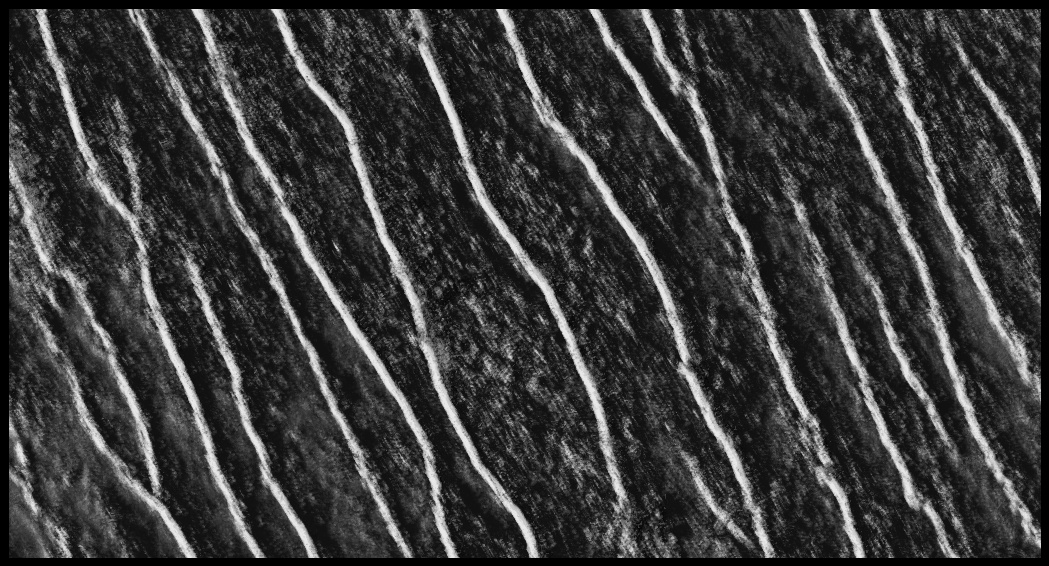
\includegraphics[width=\linewidth]{figures/KalahariSVMResponse}
		\caption{Kalahari Response Map (SVM)}
		\label{fig:kalahari_SVM_response}
	\end{subfigure}
	\begin{subfigure}{0.48\textwidth}
		\centering
		%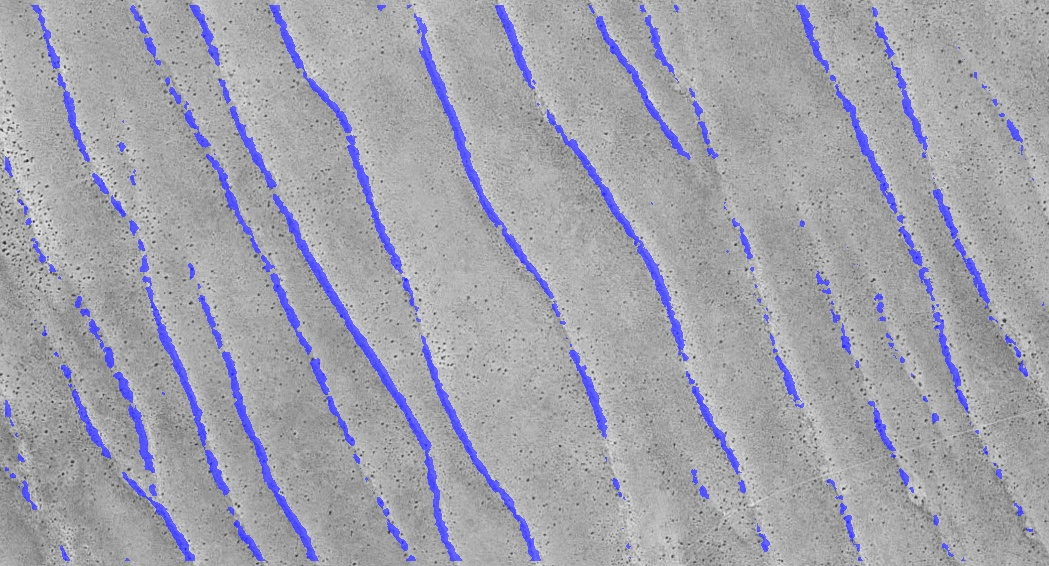
\includegraphics[width=\linewidth]{figures/KalahariSVMResults1}
		\caption{ Kalahari $R_{i,j} > 0$}
		\label{fig:kalahari_SVM_response_overlay}
	\end{subfigure}
\end{figure}
\begin{figure}[H]
	\ContinuedFloat
	\centering
	\begin{subfigure}{0.48\textwidth}
		\centering
		%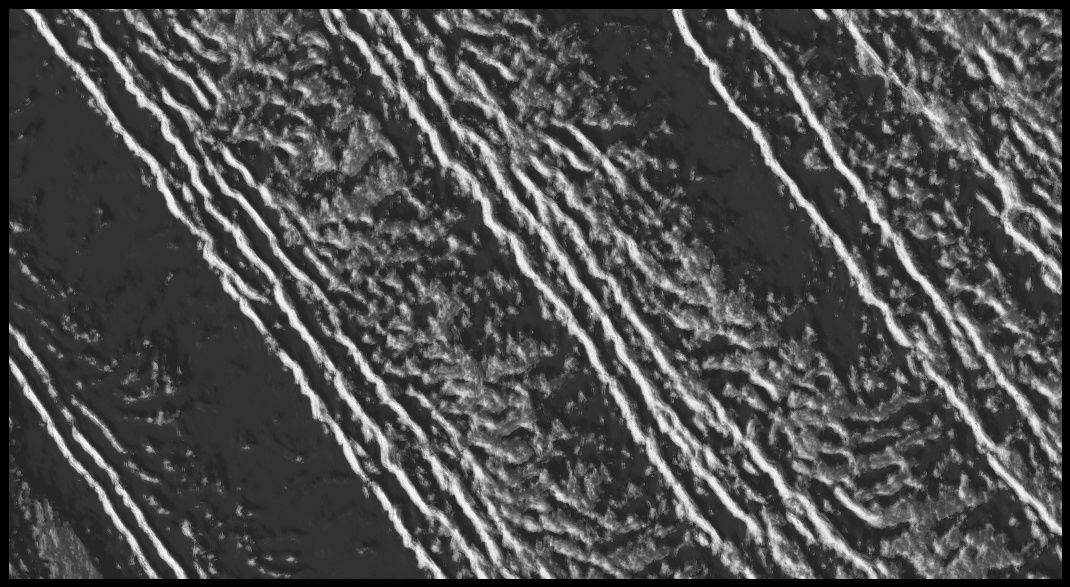
\includegraphics[width=\linewidth]{figures/NamibSVMResponse}
		\caption{Namib Response Map (SVM)}
		\label{fig:namib_SVM_response}
	\end{subfigure}
	\begin{subfigure}{0.48\textwidth}
		\centering
		%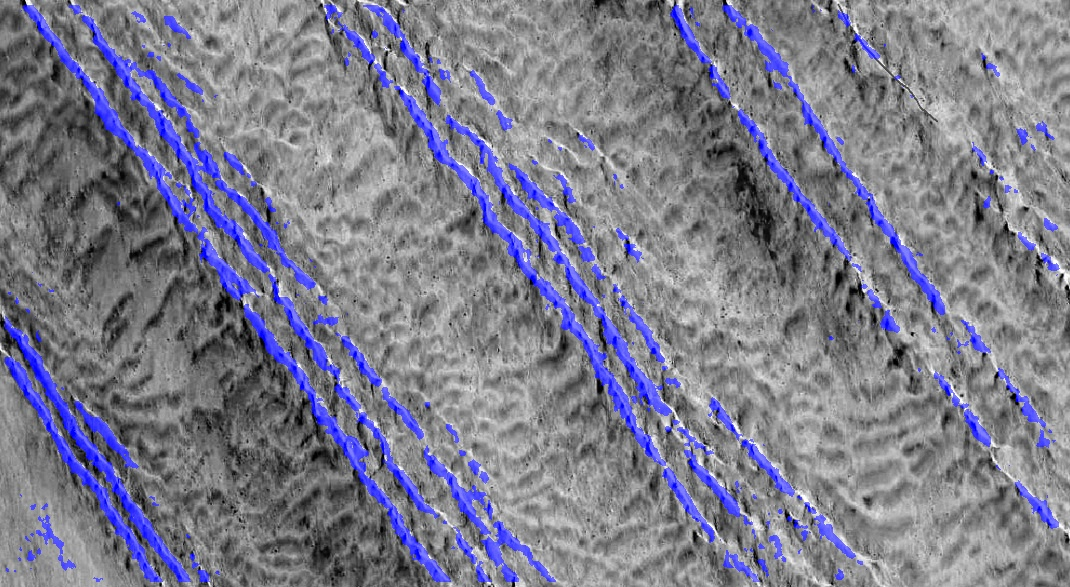
\includegraphics[width=\linewidth]{figures/NamibSVMResults1}
		\caption{ Namib $R_{i,j} > 0$}
		\label{fig:namib_SVM_response_overlay}
	\end{subfigure}
\end{figure}
\begin{figure}[H]
	\ContinuedFloat
	\centering
	\begin{subfigure}{0.48\textwidth}
		\centering
		%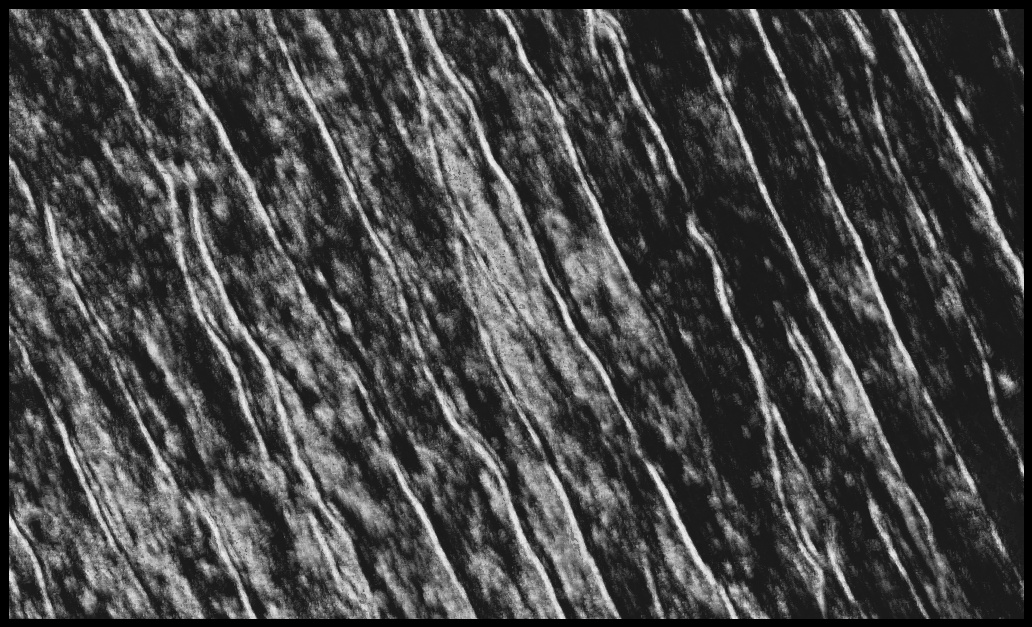
\includegraphics[width=\linewidth]{figures/SimpsonSVMResponse}
		\caption{Simpson Response Map (SVM)}
		\label{fig:simpson_SVM_response}
	\end{subfigure}
	\begin{subfigure}{0.48\textwidth}
		\centering
		%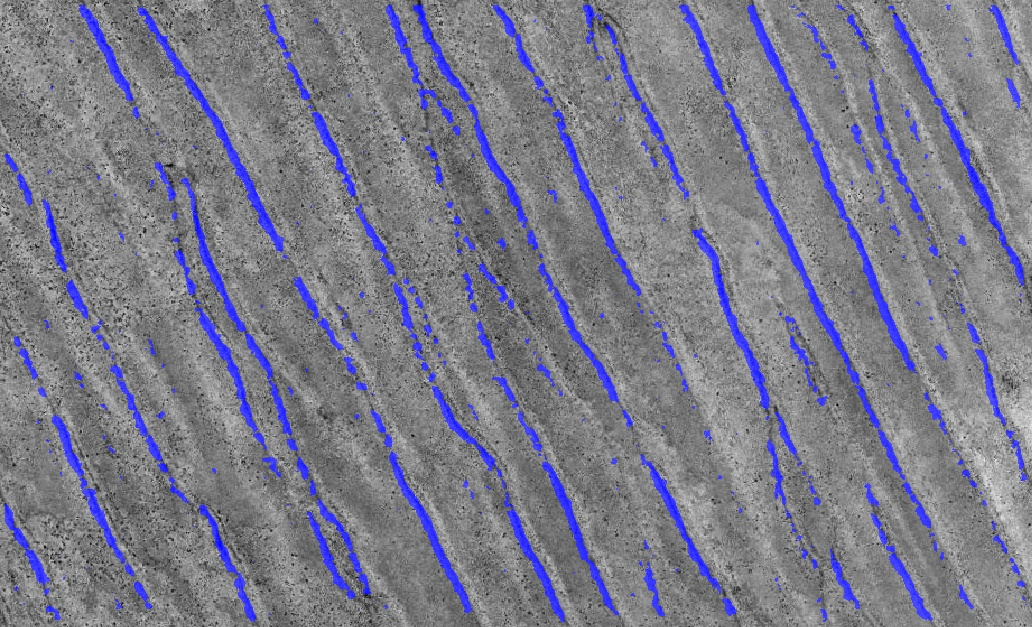
\includegraphics[width=\linewidth]{figures/SimpsonSVMResults1}
		\caption{ Simpson $R_{i,j} > 0$}
		\label{fig:simpson_SVM_response_overlay}
	\end{subfigure}
\end{figure}
\begin{figure}[H]
	\ContinuedFloat
	\centering
	\begin{subfigure}{0.48\textwidth}
		\centering
		%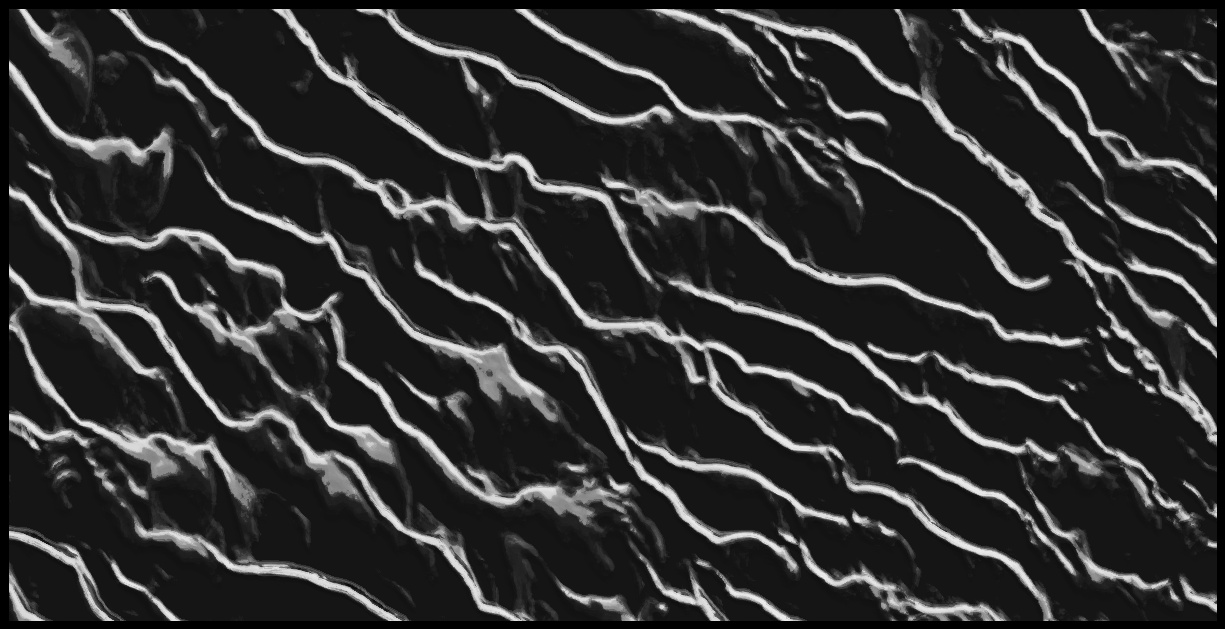
\includegraphics[width=\linewidth]{figures/SkeletonCoastSVMResponse}
		\caption{Skeleton Coast Response Map (SVM)}
		\label{fig:SkeletonCoast_SVM_response}
	\end{subfigure}
	\begin{subfigure}{0.48\textwidth}
		\centering
		%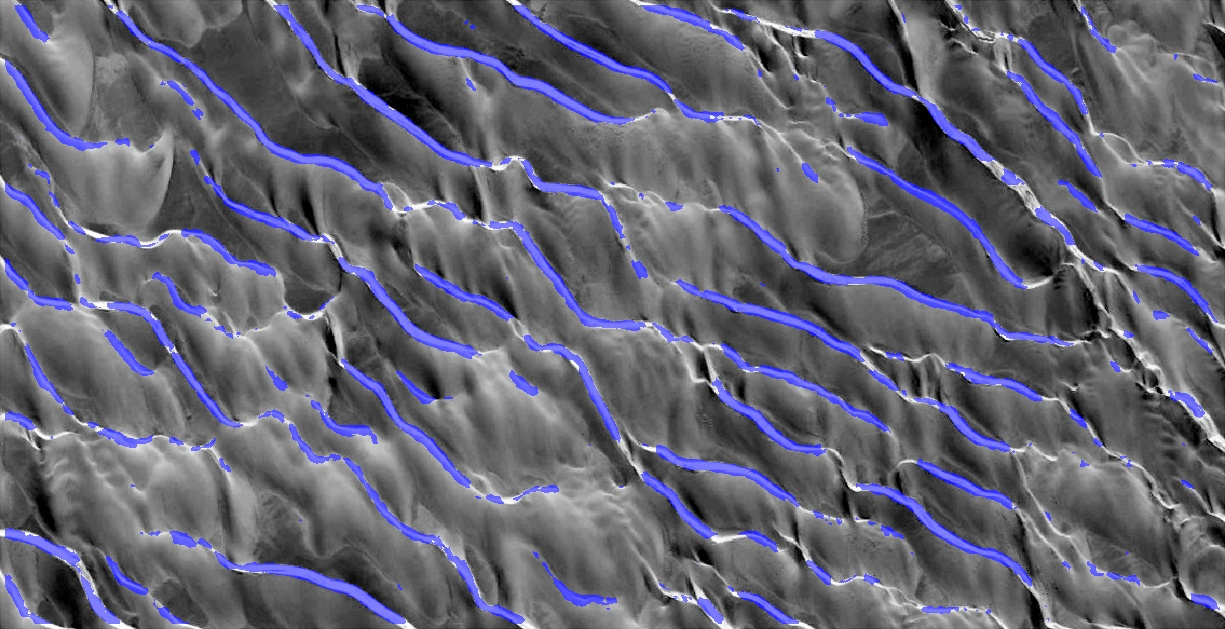
\includegraphics[width=\linewidth]{figures/SkeletonCoastSVMResults1}
		\caption{ Skeleton Coast $R_{i,j} > 0$}
		\label{fig:SkeletonCoast_SVM_response_overlay}
	\end{subfigure}
\end{figure}
\begin{figure}[H]
	\ContinuedFloat
	\centering
	\begin{subfigure}{0.48\textwidth}
		\centering
		%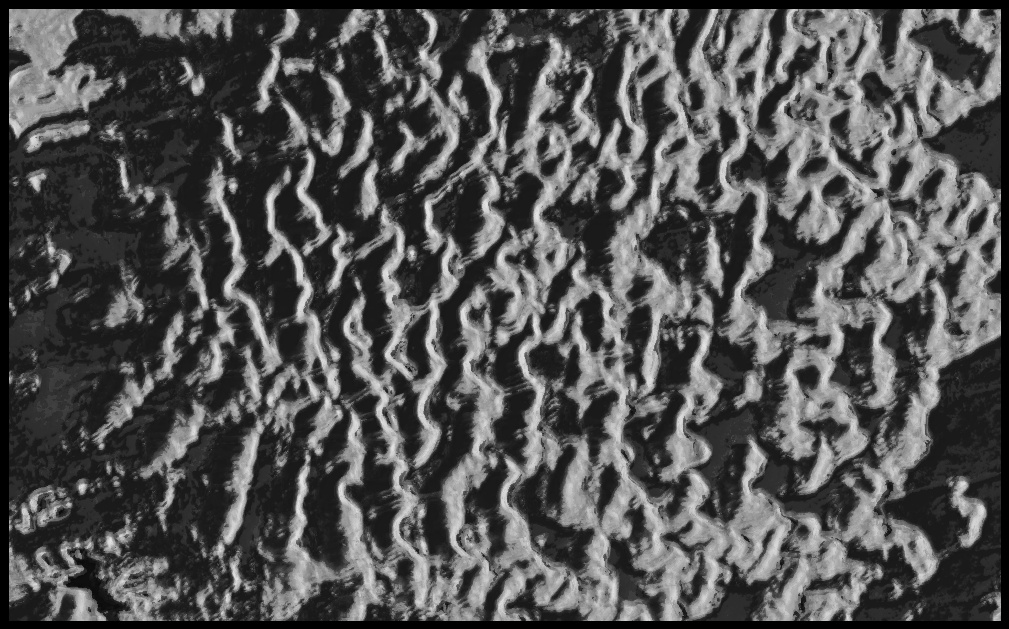
\includegraphics[width=\linewidth]{figures/WDCSVMResponse}
		\caption{WDC Response Map (SVM)}
		\label{fig:WDC_SVM_response}
	\end{subfigure}
	\begin{subfigure}{0.48\textwidth}
		\centering
		%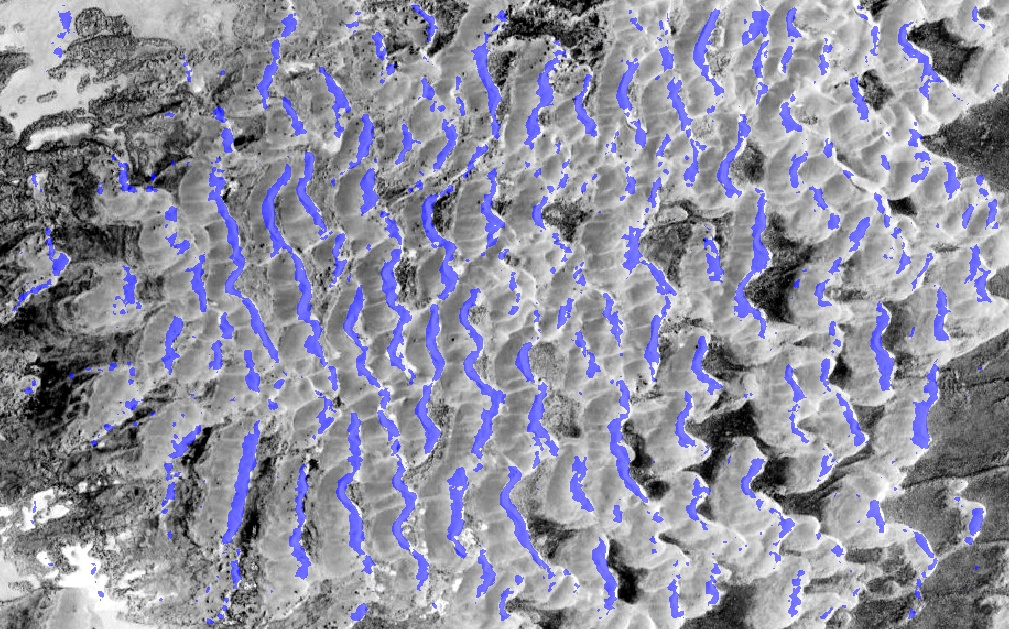
\includegraphics[width=\linewidth]{figures/WDCSVMResults1}
		\caption{ WDC $R_{i,j} > 0$}
		\label{fig:WDC_SVM_response_overlay}
	\end{subfigure}
\end{figure}
\begin{figure}[H]
	\ContinuedFloat
	\centering
	\begin{subfigure}{0.48\textwidth}
		\centering
		%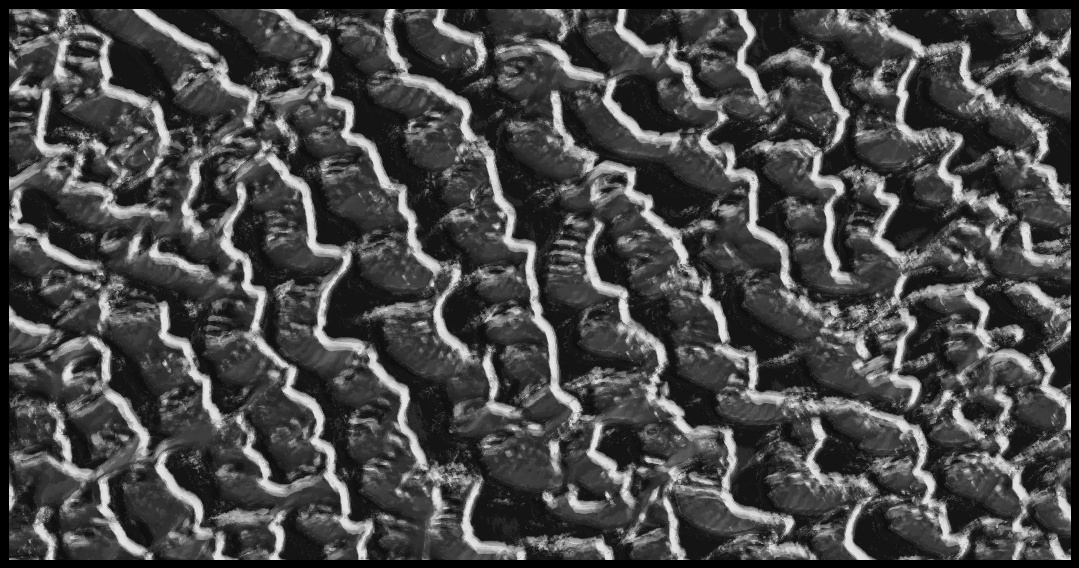
\includegraphics[width=\linewidth]{figures/WhiteSandsSVMResponse}
		\caption{White Sands Response Map (SVM)}
		\label{fig:WhiteSands_SVM_response}
	\end{subfigure}
	\begin{subfigure}{0.48\textwidth}
		\centering
		%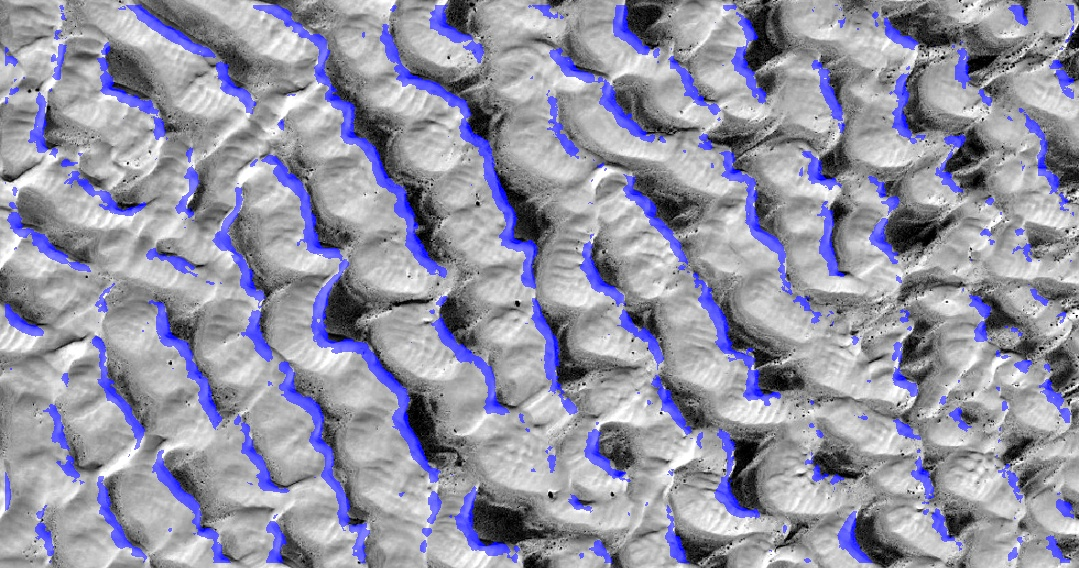
\includegraphics[width=\linewidth]{figures/WhiteSandsSVMResults1}
		\caption{ White Sands $R_{i,j} > 0$}
		\label{fig:WhiteSands_SVM_response_overlay}
	\end{subfigure}
	\caption{Results of the Support Vector Machine classifier training for crest-line identification for the Terrestrial dataset shown in Figure \ref{fig:terrestrial_dataset}. On the left is the response map (the output response of the SVM classifier using the SIFT features at each pixel). On the right, the thresholded the crest-line responses ($R_{i,j} > 0$) of the response map are overlapped on the original image. }
	\label{fig:SVM_response_results}
\end{figure}

Alternatively, the Gradient Boosted Trees classifiers seems to produce slightly smoother results. The results of the Gradient Boosted Trees classifier training are shown in Table \ref{tab:boosted_trees_training_test_results}. In Figure \ref{fig:gbt_response_results}, the response maps produced by the GBT classifier are shown, similar to Figure \ref{fig:SVM_response_results}. It is clear that the resulting response maps are generally better than the SVM model.

\begin{figure}[H]
	\centering
	\begin{subfigure}{0.48\textwidth}
		\centering
		%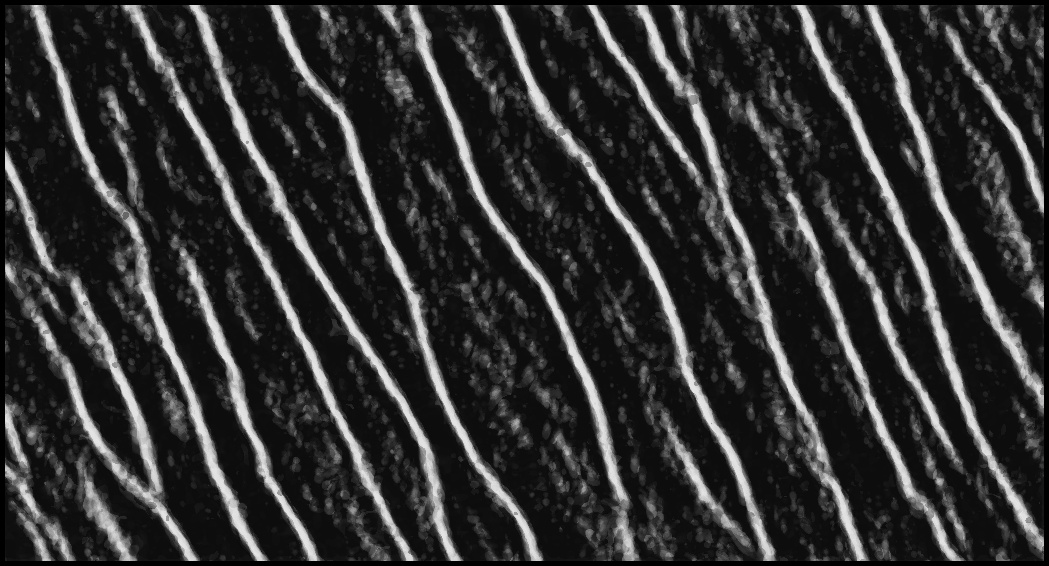
\includegraphics[width=\linewidth]{figures/KalahariGBTResponse}
		\caption{Kalahari Response Map (GBT)}
		\label{fig:kalahari_gbt_response}
	\end{subfigure}
	\begin{subfigure}{0.48\textwidth}
		\centering
		%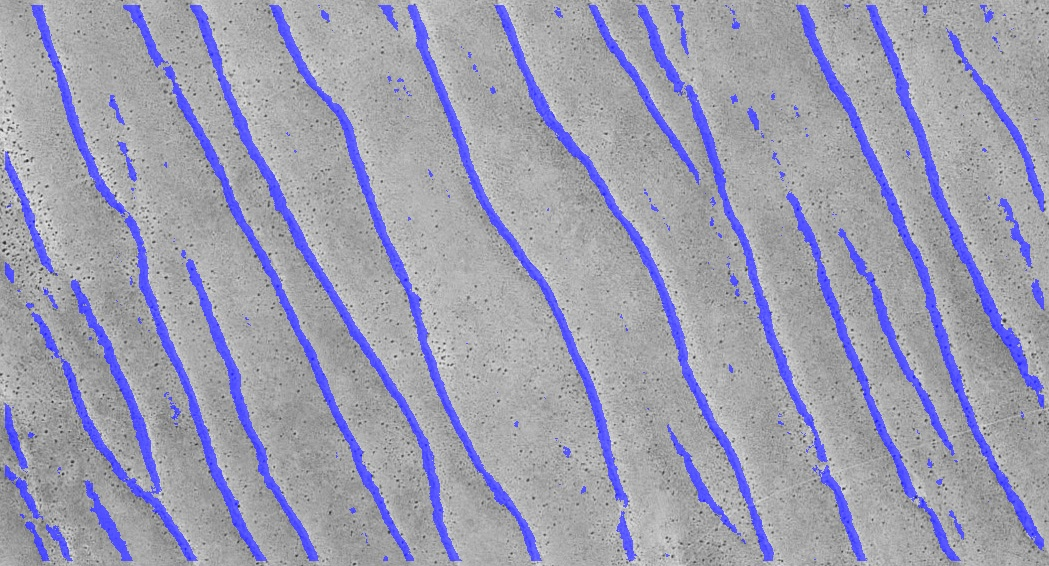
\includegraphics[width=\linewidth]{figures/KalahariGBTResults1}
		\caption{ Kalahari $R_{i,j} > 0$}
		\label{fig:kalahari_gbt_response_overlay}
	\end{subfigure}
\end{figure}
\begin{figure}[H]
	\ContinuedFloat
	\centering
	\begin{subfigure}{0.48\textwidth}
		\centering
		%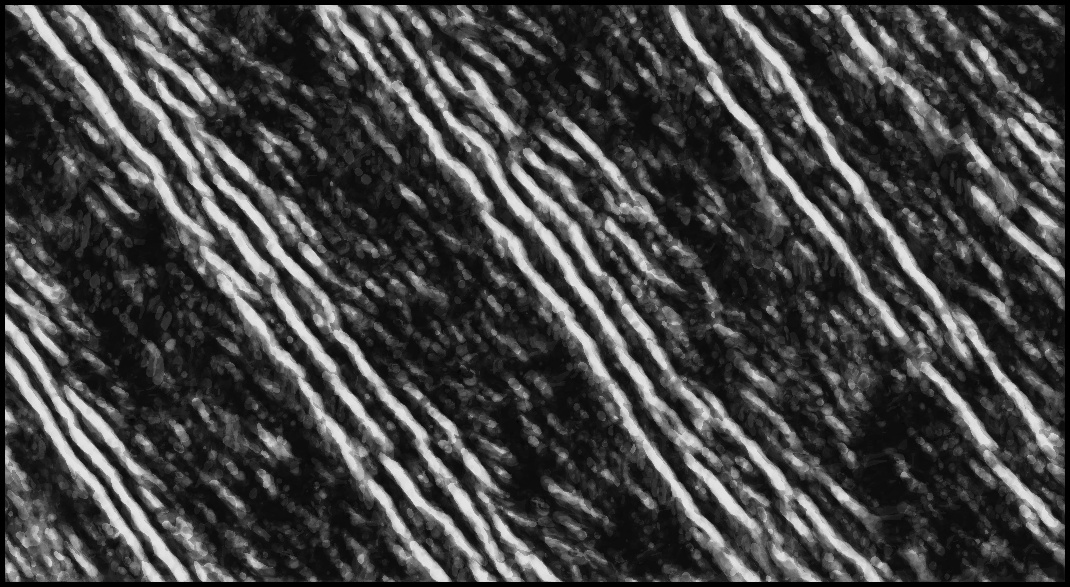
\includegraphics[width=\linewidth]{figures/NamibGBTResponse}
		\caption{Namib Response Map (GBT)}
		\label{fig:namib_gbt_response}
	\end{subfigure}
	\begin{subfigure}{0.48\textwidth}
		\centering
		%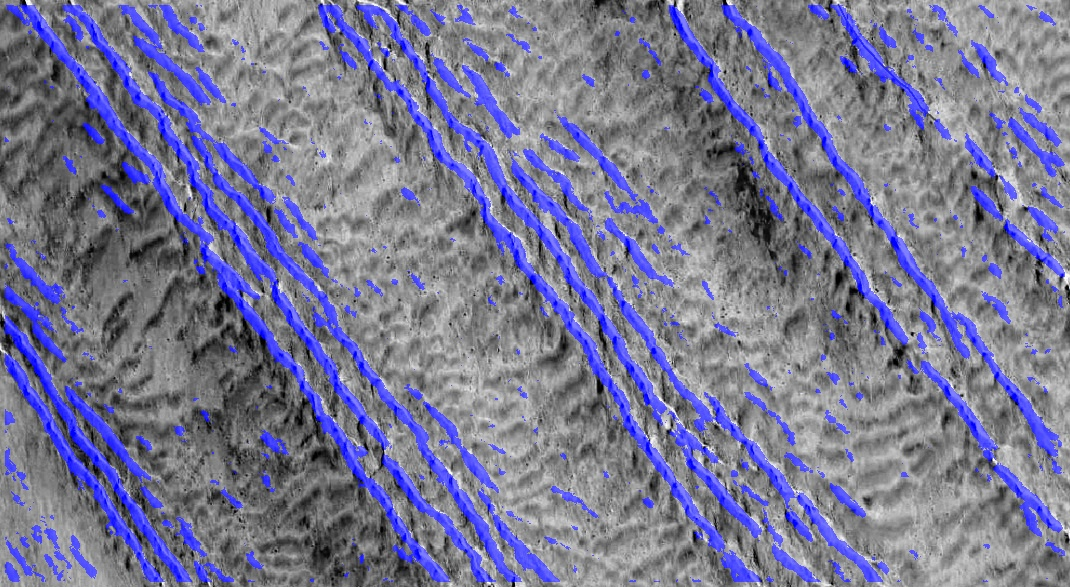
\includegraphics[width=\linewidth]{figures/NamibGBTResults1}
		\caption{ Namib $R_{i,j} > 0$}
		\label{fig:namib_gbt_response_overlay}
	\end{subfigure}
\end{figure}
\begin{figure}[H]
	\ContinuedFloat
	\centering
	\begin{subfigure}{0.48\textwidth}
		\centering
		%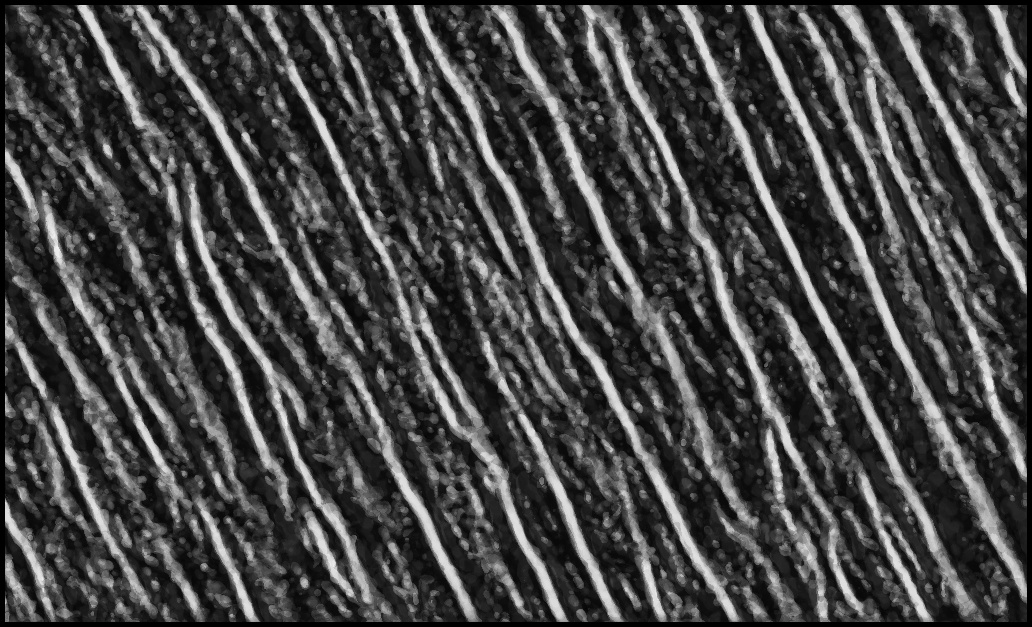
\includegraphics[width=\linewidth]{figures/SimpsonGBTResponse}
		\caption{Simpson Response Map (GBT)}
		\label{fig:simpson_gbt_response}
	\end{subfigure}
	\begin{subfigure}{0.48\textwidth}
		\centering
		%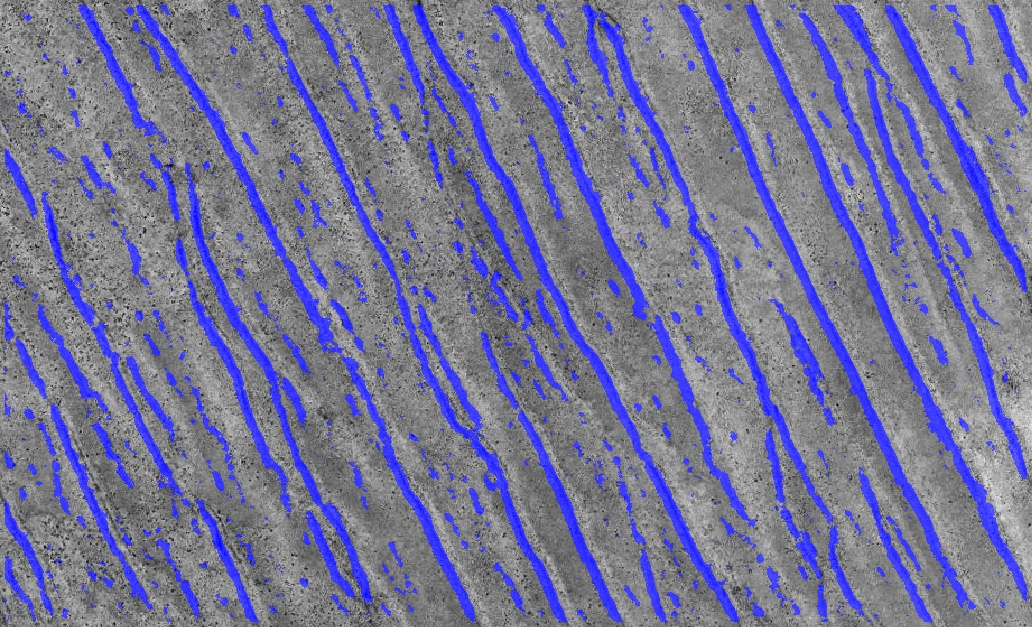
\includegraphics[width=\linewidth]{figures/SimpsonGBTResults1}
		\caption{ Simpson $R_{i,j} > 0$}
		\label{fig:simpson_gbt_response_overlay}
	\end{subfigure}
\end{figure}
\begin{figure}[H]
	\ContinuedFloat
	\centering
	\begin{subfigure}{0.48\textwidth}
		\centering
		%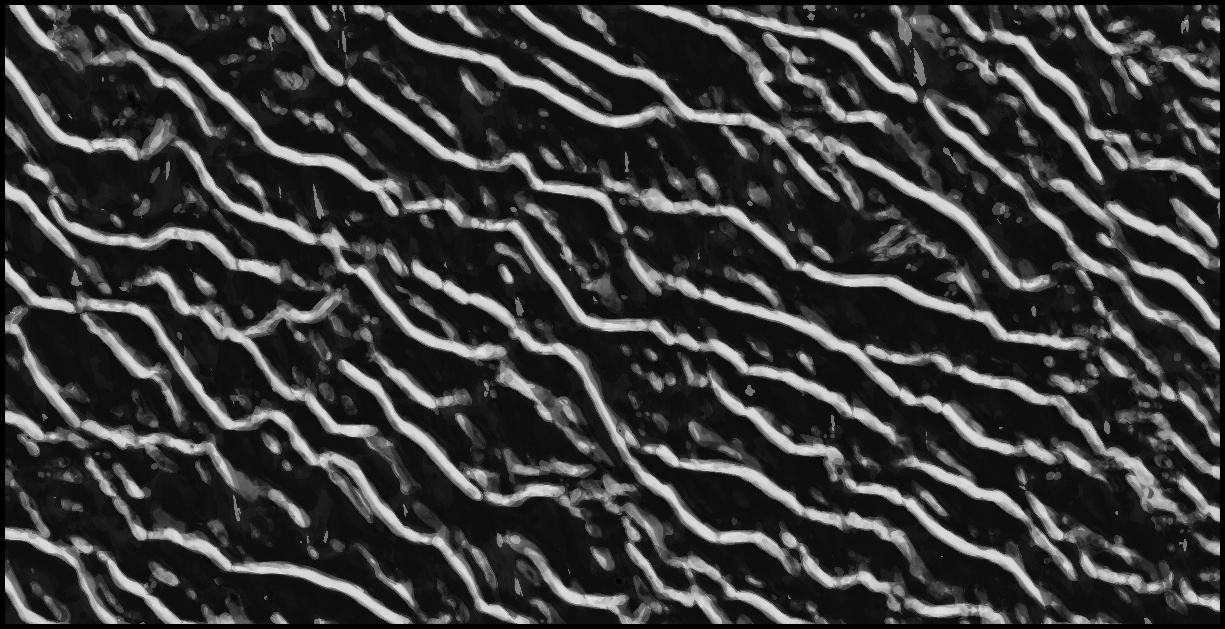
\includegraphics[width=\linewidth]{figures/SkeletonCoastGBTResponse}
		\caption{Skeleton Coast Response Map (GBT)}
		\label{fig:SkeletonCoast_gbt_response}
	\end{subfigure}
	\begin{subfigure}{0.48\textwidth}
		\centering
		%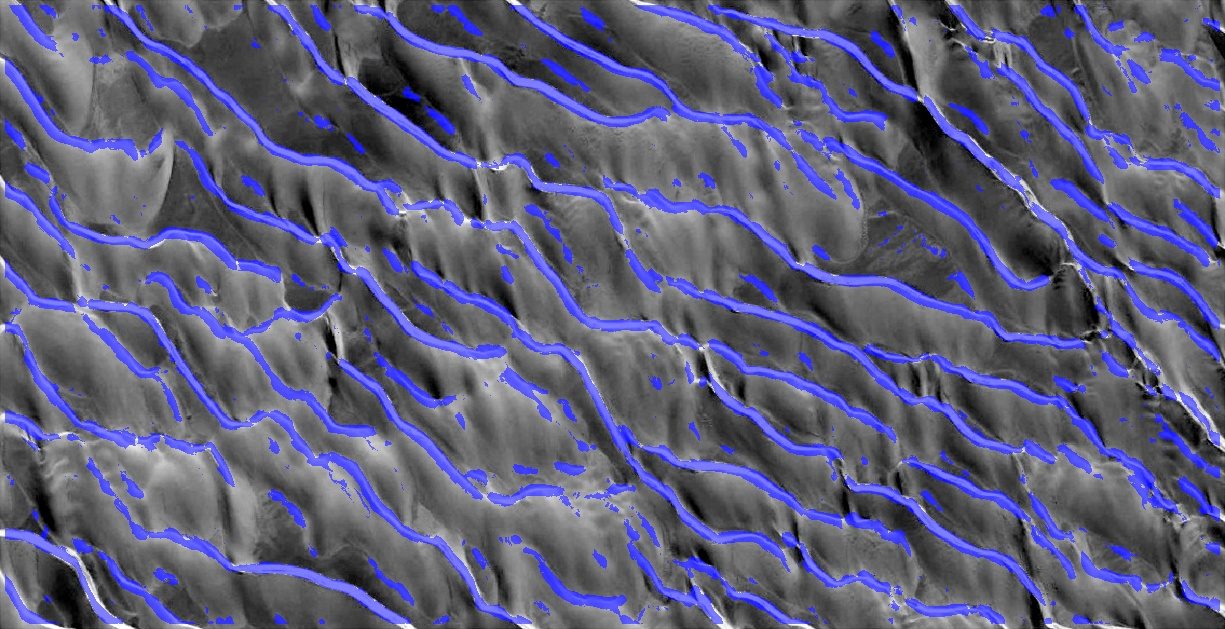
\includegraphics[width=\linewidth]{figures/SkeletonCoastGBTResults1}
		\caption{ Skeleton Coast $R_{i,j} > 0$}
		\label{fig:SkeletonCoast_gbt_response_overlay}
	\end{subfigure}
\end{figure}
\begin{figure}[H]
	\ContinuedFloat
	\centering
	\begin{subfigure}{0.48\textwidth}
		\centering
		%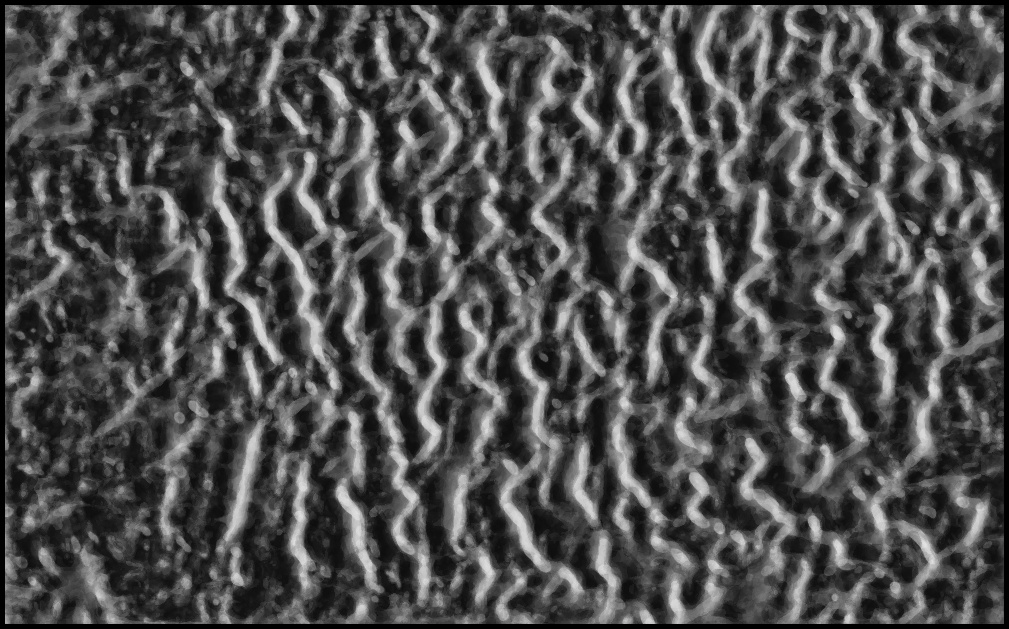
\includegraphics[width=\linewidth]{figures/WDCGBTResponse}
		\caption{WDC Response Map (GBT)}
		\label{fig:WDC_gbt_response}
	\end{subfigure}
	\begin{subfigure}{0.48\textwidth}
		\centering
		%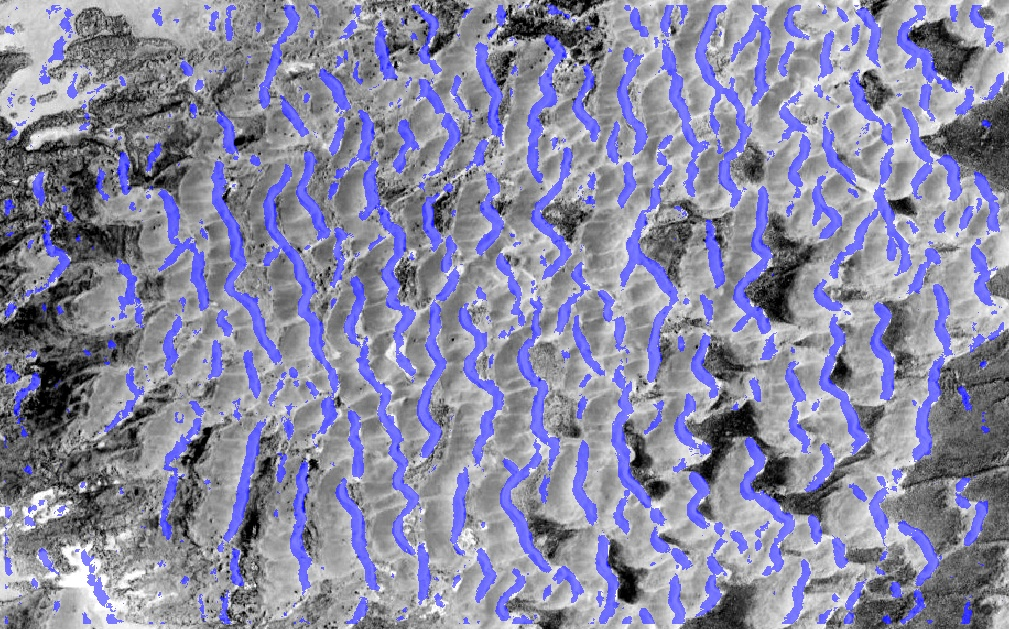
\includegraphics[width=\linewidth]{figures/WDCGBTResults1}
		\caption{ WDC $R_{i,j} > 0$}
		\label{fig:WDC_gbt_response_overlay}
	\end{subfigure}
\end{figure}
\begin{figure}[H]
	\ContinuedFloat
	\centering
	\begin{subfigure}{0.48\textwidth}
		\centering
		%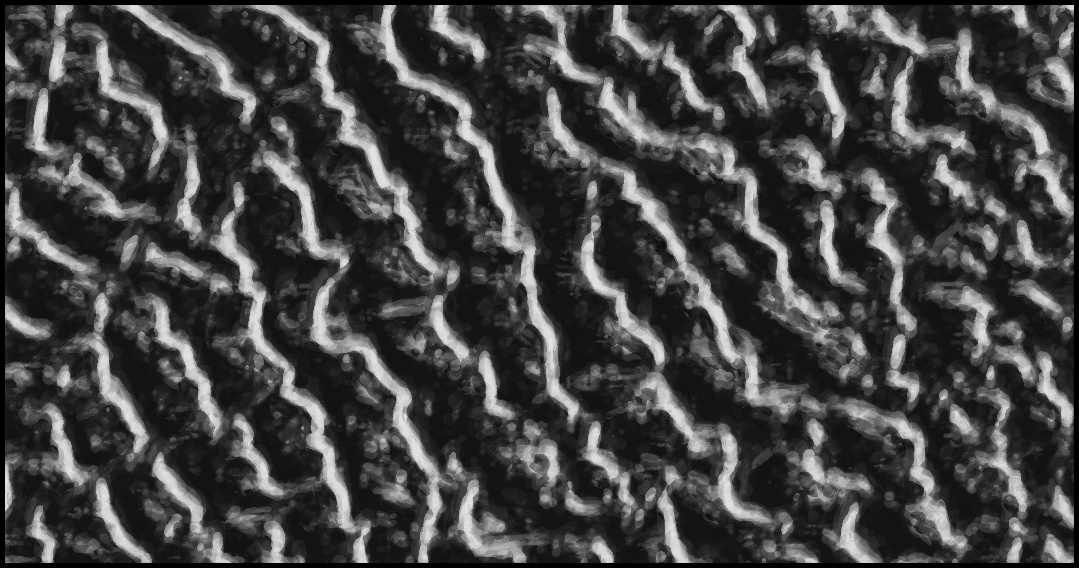
\includegraphics[width=\linewidth]{figures/WhiteSandsGBTResponse}
		\caption{White Sands Response Map (GBT)}
		\label{fig:WhiteSands_gbt_response}
	\end{subfigure}
	\begin{subfigure}{0.48\textwidth}
		\centering
		%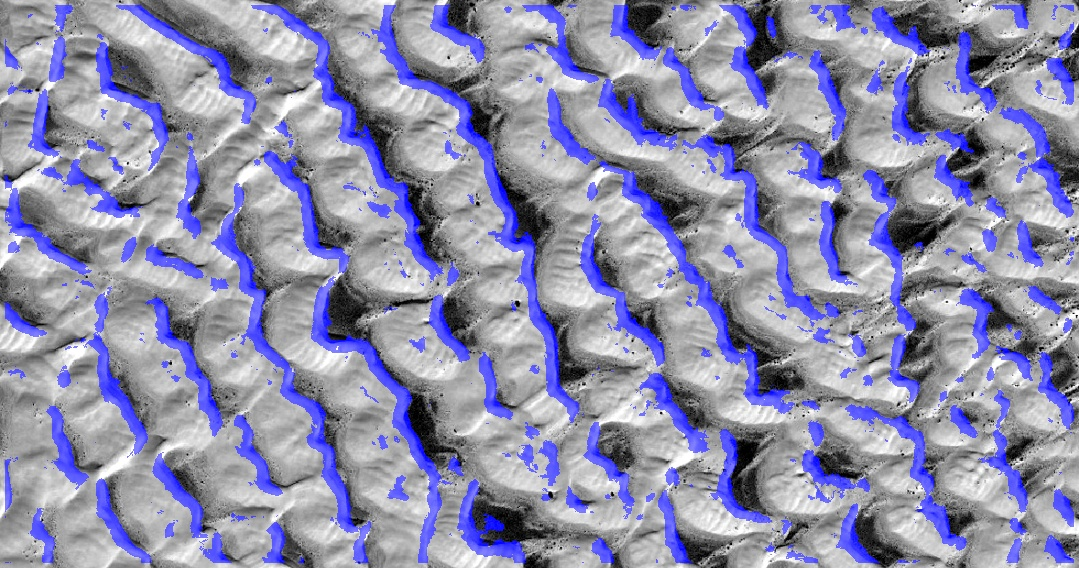
\includegraphics[width=\linewidth]{figures/WhiteSandsGBTResults1}
		\caption{ White Sands $R_{i,j} > 0$}
		\label{fig:WhiteSands_gbt_response_overlay}
	\end{subfigure}
\end{figure}
\begin{figure}[H]
	\ContinuedFloat
	\centering
	\caption{Results of the Gradient Boosted Tree classifier training for crest-line identification for the Terrestrial dataset shown in Figure \ref{fig:terrestrial_dataset}. On the left is the response map (the output response of the GBT classifier using the SIFT features at each pixel). On the right, the thresholded the crest-line responses ($R_{i,j} > 0$) of the response map are overlapped on the original image. }
	\label{fig:gbt_response_results}
\end{figure}

With the classifier model trained and the response maps generated, crest-lines can be extracted from the maps, by finding the peaks in the responses. The desired output for crest-line detection is a single pixel wide line which is smooth and contiguous. The brighter response regions tend to be thick and noisy, requiring some thinning for proper crest-line candidates to be defined. The following section will discuss the methods used to thin the responses.

\subsubsection{Crest-line Extraction: Thinning And Skeletonization}

In order to extract the desired crest-lines, the response map must be thinned. The thinning process is typically a morphological operation which reduces the thickness of a region to a single pixel width. An overview of thinning algorithms is explained in \cite{thinning-algorithms,performance-characterization-thinning,susan-new-approach-low-level-image-processing} and many other publications.

The response map should have very large values where dune crest-lines are located. The goal is to find the local maximum of the responses along ridges. The assumption is that the crest-lines should form a ridge of high response values which can be traced. As a first attempt to solve this, a recursive algorithm was created to trace the crest-lines based on the response values. The algorithm is shown in Figure \ref{fig:recursive_ridge_follow}.

\begin{figure}
	\centering
	%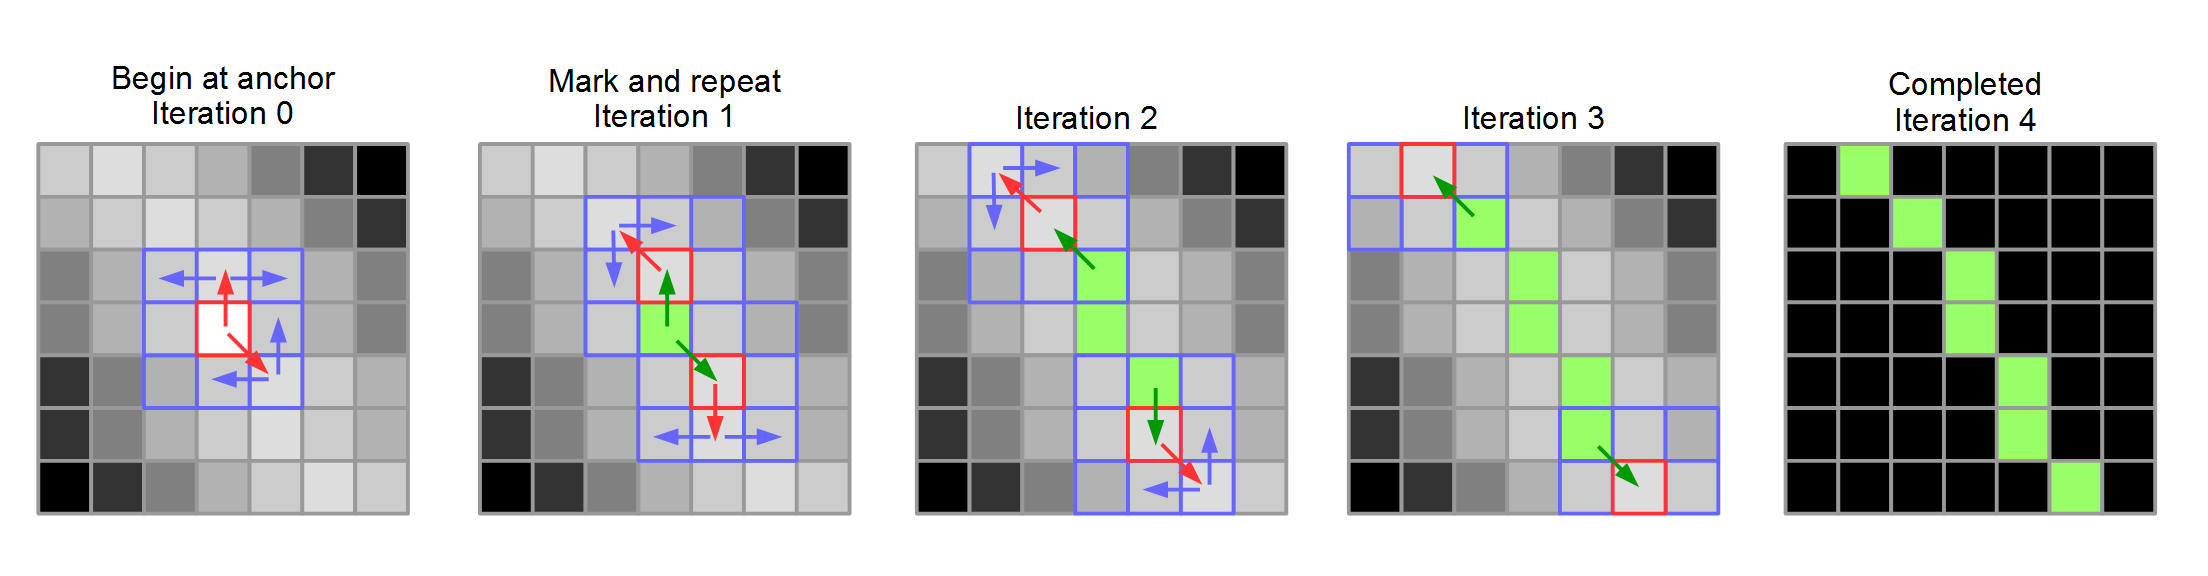
\includegraphics[width=\linewidth]{figures/SkeletonizationAlgorithm}
	\caption{A recursive algorithm for ridge following: On the first iteration, the algorithm is initialized using the detected anchor pixels, and begin search for each neighbor. Neighbors which are peaks along the ridge are used as anchors for the iteration. This algorithm recursively follows the ridge of the response images.}
	\label{fig:recursive_ridge_follow}
\end{figure}

The first step in the algorithm is to find \emph{anchor} points, which are starting points for the recursive algorithm. The so-called \emph{anchor} points are pixels for which the response value is larger than a defined threshold, and which have greater value than the eight neighboring pixels. Then, for each neighbor, a comparison in response value is done with their neighbors. If a neighbor has a response value greater than its two neighbors, then it is marked, and inserted into the queue of the recursive algorithm. The process is repeated until all ridge points are marked and the end of the ridge has been reached. Results of this process are shown in Figure \ref{fig:ridge_follow_results}.

\begin{figure}
	\centering
	\begin{subfigure}{0.48\textwidth}
		\centering
		%\includegraphics[width=\linewidth]{figures/kalahari}
		\caption{Kalahari Image}
		\label{fig:thinning_kalahari}
	\end{subfigure}
	\begin{subfigure}{0.48\textwidth}
		\centering
		%\includegraphics[width=\linewidth]{figures/thinning_kalahari_response}
		\caption{ Response Map (SIFT-GBT) }
		\label{fig:thinning_kalahari_response}
	\end{subfigure}
	\begin{subfigure}{0.8\textwidth}
		\centering
		%\includegraphics[width=\linewidth]{figures/thinning1_kalahari}
		\caption{ Ridge Following Thinning Algorithm }
		\label{fig:thinning1_kalahari}
	\end{subfigure}
	\begin{subfigure}{0.8\textwidth}
		\centering
		%\includegraphics[width=\linewidth]{figures/thinning1_kalahari_smooth}
		\caption{ Ridge Following with smoothing applied }
		\label{fig:thinning1_kalahari_smooth}
	\end{subfigure}
	\caption{The results of the recursive ridge following algorithm applied on the response map of the Kalahari image trained with the SIFT-GBT classifier. The results produced appear noisy and disjoint even with smoothing applied. }
	\label{fig:ridge_follow_results}
\end{figure}

Although the algorithm does thin the response maps, the results have a tendency to be noisy and disjoint. To remove noise, some Gaussian smoothing can be applied, which improves the noisy output, but does not resolve the issue of disjoint segments. Ideally, the crest-line segments should be contiguous segments of a certain specified size. One way to resolve this issue is to apply edge linking techniques such as defined in \cite{1986_canny_edge_detection}. No attempt to apply edge linking was made as part of this project, therefore more research could be done in to resolve the problem.

A better alternative is to use Skeletonization algorithms, such as explained in \cite{segmentation-free-skeletonization-grayscale-volumes,skeleton-pruning-contour-partitioning-discrete-curve-evolution,automatic-medial-axis-pruning-mapping-characteristics,fast-parallel-algorithm-thinning}. Skeletonization is the process of creating a skeleton (often referred to as a \emph{topological skeleton}) of an object or region. The goal of skeletonization is to shrink a region into a thin skeleton of the object or region. It is used in a variety of applications for its geometrical and topological properties. It enables the computation of features such as length, orientation, connectivity, and other features. 

The algorithm chosen to perform the thinning was the Zhang/Suen thinning algorithm from \cite{fast-parallel-algorithm-thinning}, due to it's simplicity and efficiency in implementation. Better algorithms may improve results of the thinning process, but for this application, the Zhang/Suen algorithm is sufficient. Before applying thinning to the response map, regions are created by thresholding the response map for all $R_{i,j} > 0$, as shown in Figure \ref{fig:thinning2_kalahari_threshold}. Then, the Zhang/Suen thinning algorithm can be applied to the binary image, shown in Figure \ref{fig:thinning2_kalahari}.

\begin{figure}
	\centering
	\begin{subfigure}{0.48\textwidth}
		\centering
		%\includegraphics[width=\linewidth]{figures/kalahari}
		\caption{Kalahari Image}
		\label{fig:thinning2_kalahari_input}
	\end{subfigure}
	\begin{subfigure}{0.48\textwidth}
		\centering
		%\includegraphics[width=\linewidth]{figures/thinning_kalahari_response}
		\caption{ Response Map (SIFT-GBT) }
		\label{fig:thinning2_kalahari_response}
	\end{subfigure}
	\begin{subfigure}{0.8\textwidth}
		\centering
		%\includegraphics[width=\linewidth]{figures/thinning2_kalahari_threshold}
		\caption{ Response Map Threshold $R_{i,j} > 0$ }
		\label{fig:thinning2_kalahari_threshold}
	\end{subfigure}
	\begin{subfigure}{0.8\textwidth}
		\centering
		%\includegraphics[width=\linewidth]{figures/thinning2_kalahari}
		\caption{ Zhang/Suen Thinning \cite{fast-parallel-algorithm-thinning} }
		\label{fig:thinning2_kalahari}
	\end{subfigure}
	\caption{The results of Zhang/Suen Thinning \cite{fast-parallel-algorithm-thinning} algorithm applied on the response map of the Kalahari image trained with the SIFT-GBT classifier. The output is much smoother and contiguous segments than the recursive ridge following method shown in Figure \ref{fig:recursive_ridge_follow}. }
	\label{fig:zhang_suen_results}
\end{figure}

The results shown in Figure \ref{fig:zhang_suen_results} are much better than the recursive algorithm shown in Figure \ref{fig:recursive_ridge_follow}. The skeletonization algorithm produces smooth contiguous segments which closely match the actual crest-lines. The final step of the method is to apply connected components to retrieve each dune segment. The length of each segment is measured and all segments which are shorter than a defined threshold can be filtered out as noise. 

The results of are shown in Table \ref{tab:machine_learning_approach_results}. The next section discusses a mixed approach, which combines elements and algorithms of the machine learning approach and previous approaches.



\subsection{Machine Learning and Gradient-Based Mixed Approach}\label{subsec:mixed_ml_gradient_approach}

The final approach which was studied as part of this research seeks to combine the concepts discussed in the previous approaches. From section \ref{subsection:appearance_based_approach}, the use of contours to retrieve contiguous segments is used. The dominant orientation calculation, defined in section \ref{subsec:edge_based_detection}, is also a key component in this approach. The use of gradient orientation maps defined in section \ref{subsec:gradient_orientation_based}, and the machine learning concepts presented in \ref{subsec:machine_learning_approach} are also utilized to maximize performance of crest-line detection.

\begin{figure}[H]
	\centering
	%\includegraphics[width=\linewidth]{figures/flow_mixed}
	\caption{The process flow of the machine learning and gradient-based mixed approach. The image is first preprocessed, and the machine learning model training is identical to the approach presented in \ref{subsec:machine_learning_approach}. Simultaneously, the dominant orientation is computed on the images, the gradient direction map is extracted, which is thresholded based on the dot product, and contours are extracted (in similar fashion to the approach explained in \ref{subsec:gradient_orientation_based}). Finally, the contours are filtered based on the response map, resulting in the detected crest-lines. }
	\label{fig:flow_mixed}
\end{figure}

As usual, each image is preprocessed to remove noise and enhance the image quality. From the processed images, a set of sample points of crest-lines and non-crest-lines are chosen randomly from a set of training data, as explained in section \ref{subsubsec:dataset_creation}. As we learned in sections \ref{subsubsec:feature_descriptor_extraction}, \ref{subsubsec:supervised_learning_classifiers}, and \ref{subsubsec:response_maps}, the features are extracted (SIFT), the classifier is trained (Gradient Boosted Trees), and the response map is created. The process of creating the response map is identical to the previous section, which is used to improve the localization of crest-lines.

\subsubsection{Gradient Orientation Crest-line Extraction}

In this process, extracting crest-line candidates is done using the method presented in section \ref{subsec:gradient_orientation_based}. To reiterate, the gradient orientation method computes the dominant orientation of the dune field, and computes the dot product of the gradients at each pixel with the computed dominant orientation, as shown in Figure \ref{fig:gradient_orientation_map_kalahari}. This produces an image where each pixels measures the \emph{agreement} with the dominant dune field orientation.  

\begin{figure}
	\centering
	\begin{subfigure}{0.48\textwidth}
		\centering
		%\includegraphics[width=\linewidth]{figures/kalahari}
		\caption{Kalahari Image}
		\label{fig:gradient_orientation_kalahari_input}
	\end{subfigure}
	\begin{subfigure}{0.48\textwidth}
		\centering
		%\includegraphics[width=\linewidth]{figures/gradient_direction_image}
		\caption{ Gradient Orientation Map ($D_{i,j}$) }
		\label{fig:gradient_orientation_map_kalahari}
	\end{subfigure}
	\begin{subfigure}{0.8\textwidth}
		\centering
		%\includegraphics[width=\linewidth]{figures/gradient_direction_thresholded_image}
		\caption{ Threshold for $D_{ij} > 0$ }
		\label{fig:threshold_gradient_orientation_map_kalahari}
	\end{subfigure}
	\caption{ Computing the Gradient Orientation Map \subref{fig:gradient_orientation_map_kalahari} ($D_{i,j}$) for the Kalahari image \subref{fig:gradient_orientation_kalahari_input}. The map is thresholded for all gradients which agree with the dominant orientation ($D_{ij} > 0$) in \subref{fig:threshold_gradient_orientation_map_kalahari}. The result produces smooth contiguous regions which contain candidate crest-lines. }
	\label{fig:gradient_orientation_map}
\end{figure}

The image produced, named the gradient orientation map, is thresholded resulting in a binary image containing regions which crest-line candidates. From the binary image, contours can be extracted from the regions using the same method shown in sections \ref{subsection:appearance_based_approach} and \ref{subsec:gradient_orientation_based}. The contours are typically smooth and contiguous, but result in poor localization. Also, there are two sets of contour around the regions. The goal is to therefore filter out one side of the contours, keeping only segments which land on the crest-line.

An additional step done in this approach is to improve the localization of the crest-lines based on the response map.

\subsubsection{Localization Improvement of Crest-line Segments}

As stated previously, the localization of the candidate crest-line contours do not land exactly on the crest-line ridges. We discussed in section \ref{subsubsec:gradient_magnitude_based_shift} the issue of localization of the contours, the cause of which is illustrated in Figure \ref{fig:orientation_transition_shift}. The shift explained in those sections was even more pronounced with larger values of \emph{K} (the size of the kernel used to compute the gradients), as shown in Figure \ref{fig:effect_k}. 

\begin{figure}
	\centering
	\begin{subfigure}{0.48\textwidth}
		\centering
		%\includegraphics[width=\linewidth]{figures/contour_binary_overlap}
		\caption{Kalahari Overlapped with Figure \ref{fig:threshold_gradient_orientation_map_kalahari}}
		\label{fig:kalahari_shift_overlap}
	\end{subfigure}
	\begin{subfigure}{0.48\textwidth}
		\centering
		%\includegraphics[width=\linewidth]{figures/contour_location_shift}
		\caption{ Contour Shift }
		\label{fig:contour_location_shift}
	\end{subfigure}
	\caption{ Illustration of the issue of poor localization of the extracted contours. In \subref{fig:kalahari_shift_overlap}, the binary image shown in Figure \ref{fig:threshold_gradient_orientation_map_kalahari} is overlapped on top of the Kalahari image \ref{fig:gradient_orientation_kalahari_input}. In \subref{fig:contour_location_shift}, a zoomed in image patch reveals the localization issue with the contours (shown in red) from the actual crest-line (shown in green). In order to improve the localization, the contour segments must be shifted towards crest-line. The shift is applied in the direction opposite to the computed dominant orientation. }
	\label{fig:shifting_contours_to_crest_lines}
\end{figure}

To further expand on the problem, Figure \ref{fig:shifting_contours_to_crest_lines} shows the shift created from the binary image contours. In order to improve the localization of the candidate contour segments, each segment needs to be shifted towards the crest-line ridge. The result of the contour segment extraction is shown in Figure \ref{fig:gradient_direction_results_no_shift_no_filter}, clearly showing the localization issue. Two considerations must be made in order to properly shift the candidate crest-lines to the actual crest-line: the direction of the shift, and the algorithm used to shift.

Because of the way the gradient orientation map was computed, an appropriate shifting direction can be in the opposite direction of the dominant orientation, as shown in Figure \ref{fig:contour_location_shift}. There may be better solution for shifting, but using the dominant orientation makes sense in this case and generally produces good results. Since the direction of the shift is known, the next step is to find the actual crest-line ridge along the direction of the shift. The solution proposed in \ref{subsec:gradient_orientation_based} was to find the nearest gradient magnitude peak. Unfortunately, as discussed in \ref{subsec:challenges}, some crest-line gradients may be relatively weak, making localization a difficult task.

\begin{figure}
	\centering
	\begin{subfigure}{0.48\textwidth}
		\centering
		%\includegraphics[width=\linewidth]{figures/kalahari}
		\caption{Kalahari Image}
		\label{fig:kalahari_image_2}
	\end{subfigure}
	\begin{subfigure}{0.48\textwidth}
		\centering
		%\includegraphics[width=\linewidth]{figures/gradient_direction_results_no_shift_no_filter}
		\caption{Contours Extracted from Binary Image}
		\label{fig:gradient_direction_results_no_shift_no_filter}
	\end{subfigure}
	\begin{subfigure}{0.48\textwidth}
		\centering
		%\includegraphics[width=\linewidth]{figures/gradient_direction_results_no_filter}
		\caption{ After Applying Shift }
		\label{fig:gradient_direction_results_no_filter}
	\end{subfigure}
	\begin{subfigure}{0.48\textwidth}
		\centering
		%\includegraphics[width=\linewidth]{figures/gradient_direction_shift_results}
		\caption{ Filtering Based on Responses }
		\label{fig:gradient_direction_shift_results}
	\end{subfigure}
	\caption{ The process of extracting candidate crest-lines using the gradient orientation map, and the machine learning approach. The Kalahari input image shown in (a), is processed to extract contours shown in (b). A shift towards the nearest peak in response values is applied (c), and all segments which have low responses are filtered out in (d). The color scheme shown in (b-d) is true positive crest-lines detections (green), the positive identified ground truth (blue), false negatives (yellow), and false positives (red).}
	\label{fig:shifting_contours_results}
\end{figure}

Therefore, using the response map computed in the previous approach seems to be an appropriate way to resolve this problem. The response map will have larger values where crest-lines are located. So, the shift can be determined by doing a search along the opposite direction of the dominant orientation, and finding peaks in the response map. The shift can then be applied based on the computed distance, for each point along the contour segments. Smoothing can be applied in order to ensure that segments remain contiguous after the shift is applied. The results of the shift are shown in Figure \ref{fig:gradient_direction_results_no_filter}.

Once the shift has been applied to every contour segments, filtering non-crest-line segments can be done by simply removing all contour segments which fall on weak responses. After all contours have been filtered, the remaining segments can be further filtered by segment length. All segments which are too short are removed from candidate crest-line segments. The output of this process is shown in Figure \ref{fig:gradient_direction_shift_results}.

Overall, the mixed machine learning and gradient orientation based method produced excellent results in most cases but struggled on more complex dune systems. Section \ref{subsec:results-and-discussion} summarizes the results of this approach on both our dataset and the dataset provided by \cite{vaz_object_based_dune_analysis}. The next section discusses the method and metrics computed from the detected crest-lines.


\subsection{Dune Field Morphology Metrics} \label{subsec:dune-field-metrics}
The final step of the process is to extract meaningful features and metrics for researchers to study from the dune fields. This process requires a good set of detected crest-lines. The output crest-line segments extracted in the previous methods are used as input for computing the features.

There are many features metrics of interests to scientists in this field, including dune spacings, orientation, shape, size, length, bifurcations, and many more. These metrics can be used to study and understand the movements of various patterns of dunes over time in a specific area.

As part of this research, we focused mainly on orientation and spacing of dunes, and used those metrics as validations for the effectiveness of the dune detection methods. Although these metrics are not a complete evaluation of the dune field, they are sufficiently complex to provide valuable feedback for scientists.

\subsubsection{Dune Field Orientation Computation}
One may argue that the orientation of the dune field could be simply computed in the same manner as explained in section \ref{subsec:edge_based_detection}. However, a more generalized approach is preferred which computes the metrics from any set of two dimensional points, regardless of the input image. 

In order to compute the average dune field orientation from the detected points, the data must be formated appropriately. The detected crest-lines are typically a set of two dimensional points on the image. These points form lines and segments of various shapes and lengths. The simplest way to compute the orientation is to fit lines to each segments and compute the average orientation of the lines.

There are many commonly used methods to fit lines to segments. One popular method is the Hough Transform initially proposed in \cite{hough-1959-paper,hough-1962-patent,hough-duda-1972-paper}, which searches a space of parameters voting for segments which contribute to the line. The Hough transform can be generalized to many shapes suchs as circles and ellipses, but the parameter space gets much larger for complex shapes. The main drawback of the Hough transform is the computational cost of search a large parameter space.

An alternative method is the Ramer-Douglas-Peucker algorithm, proposed in \cite{ramer-1972-paper,douglas-peucker-1973-paper,douglas-hershberger-snoeyink-1992-paper}, with the implementation provided within the OpenCV (\cite{opencv_library}) framework. The method is used for simplifying or approximating any given curve to a subset of points. Thus, the dune segments can be reduced to subset of lines. The only parameter required is the allowable error in the approximation. Larger values allow more deviation, producing longer coarse approximations of the segments, while smaller values approximate the curve more closely, producing short segments which are sensitive to noise. The parameter is chosen to produce optimal results for the application.

\begin{figure}
	\centering
	\begin{subfigure}{0.48\textwidth}
		\centering
		%\includegraphics[width=\linewidth]{figures/SegmentationTestImage}
		\caption{Sample Test Image}
		\label{fig:connected_component_test_image}
	\end{subfigure}
	\begin{subfigure}{0.48\textwidth}
		\centering
		%\includegraphics[width=\linewidth]{figures/SegmentationTestResult}
		\caption{Connected Components Labeling}
		\label{fig:connected_component_test_results}
	\end{subfigure}
	
	\caption{ The connected component algorithm applied a sample test image \subref{fig:connected_component_test_image}. The results \subref{fig:connected_component_test_results} show that segments can be extracted correctly. }
	\label{fig:connected_component_test}
\end{figure}

Another critical requirement for this algorithm to work is the fact that each segment must be a single contiguous line or curve. This means that any segments extracted from the connected components algorithm (\cite{connected-components-samet-tamminen-1988-paper,connected-components-dillencourt-1992-paper}) must be sorted and organized in a list to ensure contiguous segments of points. All forks and bifurcations are detected and split into separate segments. The labeling of segment is demonstrated on a test image shown in Figure \ref{fig:connected_component_test}. The results in Figure \ref{fig:connected_component_test_results} show that these segments can be extracted and split into many single line segments. Although the algorithm may not produce optimal results, the output is sufficient for this application.

Once the segments have been extracted and sorted, the line fitting algorithm presented in \cite{ramer-1972-paper} can be applied. The result is a set of lines, which can be represented as vectors contain the position and orientation of each line. The orientation components are used to compute the average orientation of the dune field.

As explained in \cite{computing-average-orientation-of-vectors}, computing the average orientation of vectors is not as trivial as simply averaging the orientations. To illustrate the problem, the average of an angle of $350^{\circ}$ and $10^{\circ}$ would be $180^{\circ}$, when in fact a more appropriate average should be $0^{\circ}$. Averaging may produce an adequate approximation, but the von Mises distribution based method proposed in \cite{computing-average-orientation-of-vectors} typically produces much more accurate results. Therefore, this technique is used to compute the average orientation of the lines.

With the orientation of the dune field computed, the average dune distance can then be computed.

\subsubsection{Inter-Dune Distance Computation}
Computing the distance between crest-lines is a feature interesting to many researchers in the field. For simplicity, the inter-dune spacing is computed for the entire dune field image. The resulting measurement is in pixels in our case, but, if the scale of the satellite image is known (meters per pixels), then the measurement can be easily converted to a real world measurement. There are many ways to compute the inter-dune distance, but in this approach the simplest way was used, shown in Figure \ref{fig:inter-dune-distance-computation}. 

\begin{figure}
	\centering
	%\includegraphics[width=\linewidth]{figures/DuneMetrics}
	\caption{ Computing the inter-dune distance using the average orientation. Once the average orientation has been computed, the inter-dune distance can be computed by measuring the distance between segments along an orthogonal axis to the average orientation.}
	\label{fig:inter-dune-distance-computation}
\end{figure}

Using the binary image of the extracted dune crest-lines, and the average orientation computed, an iterative approach is used to measure the distance between the dunes. A search is done at each pixel along an orthogonal axis from the average orientation. When a crest-line is hit, the number of pixels traveled are counted until another dune is found. The process is repeated for the entire binary image. The lengths are averaged resulting in the average dune spacing for the entire dune field.

The results produced may not be optimal and accurate but can be used as an indicator to evaluate the effectiveness of the dune crest-line detections. The results and metrics are presented in section \ref{subsec:results-and-discussion}.










